% !TeX spellcheck = eu_ES
\documentclass[eu]{ifirak}\usepackage[]{graphicx}\usepackage[]{color}
%% maxwidth is the original width if it is less than linewidth
%% otherwise use linewidth (to make sure the graphics do not exceed the margin)
\makeatletter
\def\maxwidth{ %
  \ifdim\Gin@nat@width>\linewidth
    \linewidth
  \else
    \Gin@nat@width
  \fi
}
\makeatother

\definecolor{fgcolor}{rgb}{0, 0, 0}
\newcommand{\hlnum}[1]{\textcolor[rgb]{0.659,0.4,0.051}{#1}}%
\newcommand{\hlstr}[1]{\textcolor[rgb]{0.659,0.4,0.051}{#1}}%
\newcommand{\hlcom}[1]{\textcolor[rgb]{0.333,0.533,0.09}{#1}}%
\newcommand{\hlopt}[1]{\textcolor[rgb]{0,0,0}{#1}}%
\newcommand{\hlstd}[1]{\textcolor[rgb]{0,0,0}{#1}}%
\newcommand{\hlkwa}[1]{\textcolor[rgb]{0.133,0.224,0.659}{\textbf{#1}}}%
\newcommand{\hlkwb}[1]{\textcolor[rgb]{0.549,0.114,0.412}{\textbf{#1}}}%
\newcommand{\hlkwc}[1]{\textcolor[rgb]{0.659,0.573,0.133}{\textbf{#1}}}%
\newcommand{\hlkwd}[1]{\textcolor[rgb]{0.659,0.133,0.482}{#1}}%

\usepackage{framed}
\makeatletter
\newenvironment{kframe}{%
 \def\at@end@of@kframe{}%
 \ifinner\ifhmode%
  \def\at@end@of@kframe{\end{minipage}}%
  \begin{minipage}{\columnwidth}%
 \fi\fi%
 \def\FrameCommand##1{\hskip\@totalleftmargin \hskip-\fboxsep
 \colorbox{shadecolor}{##1}\hskip-\fboxsep
     % There is no \\@totalrightmargin, so:
     \hskip-\linewidth \hskip-\@totalleftmargin \hskip\columnwidth}%
 \MakeFramed {\advance\hsize-\width
   \@totalleftmargin\z@ \linewidth\hsize
   \@setminipage}}%
 {\par\unskip\endMakeFramed%
 \at@end@of@kframe}
\makeatother

\definecolor{shadecolor}{rgb}{.97, .97, .97}
\definecolor{messagecolor}{rgb}{0, 0, 0}
\definecolor{warningcolor}{rgb}{1, 0, 1}
\definecolor{errorcolor}{rgb}{1, 0, 0}
\newenvironment{knitrout}{}{} % an empty environment to be redefined in TeX

\usepackage{alltt}

\usepackage{amsmath,latexsym,amssymb,natbib}
\usepackage{listings}
\usepackage{ifcommands,subfigure}
\usepackage[T1]{fontenc}
\usepackage{tcolorbox}

\newcommand{\zkk}{\guillemotleft}
\newcommand{\skk}{\guillemotright}
\newcommand{\code}[1]{\texttt{#1}}
\IfFileExists{upquote.sty}{\usepackage{upquote}}{}
\begin{document}
\ikasturtea{2013/2014}
\irakasgaia{Bilaketa Heuristikoak}
\title{BHLN: Oinarrizko Kontzeptuak}
\date{}
\irakaslea{Borja Calvo, Usue Mori}
\author{Borja Calvo, Josu Ceberio, Usue Mori}





\tel{943 01 50 13}
\mail{borja.calvo@ehu.es}


\maketitle

\begin{abstract}
Lehenengo kapitulu honetan optimizazioaren ikuspen globala aurkeztuko dugu, oinarrizko kontzeptuak azalduz. Kapitulua bi zatitan dago banatuta; lehenengoan optimizazio problemak izango dira aztergai eta, bereziki, hauen konplexutasuna, hau baita metodo heuristikoak erabiltzeko motibaziorik garrantzitsuena. Heuristikoak dira, bigarren zatiaren protagonistak. Zehazki, heuristikoak diseinatzeko eta erabiltzeko kontuan eduki beharreko kontzeptuak aztertuko ditugu. 
\end{abstract}

\section{Sarrera}

Optimizazioa oso kontzeptu hedatua da, askotan baitarabilgu --konturatu barik bada ere--. Problema baten aurrean \textit{soluzio ezberdinak} daudenean, soluzio horien \textit{kalitatea} neurtzeko eraren bat izanez gero, \textit{soluziorik onena} bilatzea izango da optimizazioaren helburua. Definizio orokor honetan problema mota asko sartzen dira. Alabaina, liburu honetan \textit{optimizazio konbinatorioa} deritzon problematan zentratuko gara, gehien bat. Optimizazio problemak aspalditik aztertuak izan arren, matematika aplikatuan berriki bereizi den arloa da optimizazioa.
 

\subsection{Hastapen historikoa}
I Munduko Gerra amaitu zenean garaileek Alemaniari oso baldintza gogorrak inposatu zizkioten Versalles-eko itunean; besteak beste, Alemaniak armada izatea zeharo debekatuta zeukan. Hare gehiago, itun honek jasotzen zituen baldintza ekonomikoak zirela eta hogeigarren hamarkadan Alemaniako egoera nahiko larria zen; hala ere, krisi momentu horretan, pertsona batek promes egin zuen herrialdea larrialdi horretatik aterako zuela... Pertsona hori Hitler zen eta 1933an hauteskundeak irabaziz boterea lortu zuen; orduan, II Munduko Gerran amaituko zuen gertakizun sekuentzia hasi zen.

1934. urtean Hitler-ek Alemaniako berrarmatze prozesua agindu zuen, eta 1935eko udaberrirako bere aireko armada --Luftwaffea-- Britainiakoaren parekoa zela aldarrikatzen hasi zen. Nazien hegazkin bonbaketarien mehatxua arazo larri bihurtu zen Britaniko Gobernuarentzat eta, hortaz, aire defentsa antolatzeari ekin zion. Aireko estatu-idazkariak \zkk Imperial College of Science and Technology\skk -ko errektoreari aireko defentsaren arazoa aztertuko zuen batzordea sortzea eskatu zion; batzorde honen lanaren ondorioz, 1935eko udan radarra asmatu zuen Robert Watson-Watt-ek. Tresna oso erabilgarria izan arren, zuen ahalmen guztia ateratzeko, defentsa sisteman --behatokiak, ehiza-hegazkinak, antiaereoko artilleria, ...--  integratu beharra zegoen: alabaina, laster hau erraza ez zela izango konturatu ziren arduradunak. Izan ere, defentsa operazioen antolakuntza, bere osotasunean, oso arazo konplexua zen. Hori dela eta, problema hau ikuspegi matematikotik ikertzen hasi ziren; Ikerkuntza Operatiboa sortu zuten.

II Munduko Gerran zehar operazioen antolakuntza \zkk matematikoa\skk k arrakasta handia izan zuen Britaniko armadan eta, hortik, Estatu Batuetako armadara hedatu zen. 1945ean gerra amaitu zenerako, mila pertsonatik gora zeuden Ikerkuntza Operatiboan lanean Britaniko armadan.

Gerra amaitu ostean, Europako herrialdeen egoera oso larria zen: herrialdeak suntsituta, baliabideak gerran xahututa, ... Hurrengo urteetan, herrialdeak berreraikitzeko erronkari aurre egiteko, gerra bitartean operazio militarrak antolatzeko garatutako metodologia matematikoak bereziki egokiak zirela konturatu ziren agintariak. Adibide gisa, Dantzigek --gerran US armadan ziharduena-- 1947an Ikerkuntza Operatiboko algoritmorik ezagunena, Simplex algoritmoa, proposatu zuen. 

Arlo berri honek ikertzaileen arreta erakarri zuen eta asko hedatu zen gerraosteko garaian. Hasierako urteetan planteatzen ziren algoritmoek soluzio zehatzak lortzea zuten helburu baina teknika hauek problema mota konkretuak ebazteko bakarrik erabili zitezkeen --problema linealak, adibidez--. Hirurogeita hamarreko hamarkadan zientzialariek problemen konplexutasuna aztertzeari ekin zioten. Bestalde, konputagailu pertsonalak agertu ziren merkatuan. Problema batzuentzat konplexutasun + tamaina konbinaketa zela eta soluzio zehatza lortzea ezinezkoa zen. Gauzak horrela, merkatuan algoritmo heuristikoak agertzen hasi ziren zeinek, soluzio zehatza ez bermatu arren, soluzio onak ematen zituzten denbora laburrean.

Metodo heuristikoak oso interesgarriak ziren, baina desegokiak problema berrietan berrerabiltzeko. Hori dela eta, 1975etik aurrera beste hurbilketa batzuk, bilaketa heurisktikoak edo metaheuristikak deritzenak, garatzen hasi ziren. Ona hemen adibide eta data batzuk:

\begin{itemize}
\item 1975 - John Hollandek algoritmo genetikoak proposatu zituen
\item 1977 - Fred Gloverrek \textit{scatter search} algoritmoa proposatu zuen
\item 1983 - Kirkpatrick eta lankideak \textit{simulated annealing} algoritmoa proposatu zituzten
\item 1986 - Fred Gloverrek tabu bilaketa algoritmoa proposatu zuen
\item 1986 - Gerardo Beniek eta Jing Wangek \textit{swarm intelligence} kontzeptua proposatu zuten
\item 1992 - Marco Dorigoek \textit{Ant Colony Optimization} (ACO) algoritmoa proposatu zuen
\item 1996 - Muhlenbeinek eta Paassek \textit{Estimation of Distribution Algorithms} (EDAs) kontzeptua proposatu zuten
\end{itemize}

\section{Optimizazio problemak}\label{sec:opt_problemak}

Egunero erabakiak hartzen dira; enpresatan, zientzian, industrian, administrazioan, ... Erabaki-hartzea nonahi dago eta, geroz eta konpetitiboagoa den gure munduan, prozesu hori arrazionalki hurbiltzeko beharra daukagu. 

Erabaki-hartzea hainbat pausutan bana daiteke. Lehendabizi, problema formalizatu behar da, gero matematikoki modelatu ahal izateko. Behin problema modelaturik, soluzio onak topatu behar ditugu problemarako --erabaki optimoa, alegia--. 

Problema erreal batean dihardugunean, hartutako erabakia optimoak praktikan jarri beharko genituzke, egiaztatzeko ea funtzionatzen dutenetz; arazoren bat egonez gero, atzera jo beharko genuke problemaren formulazioa berrikusteko.

\begin{tcolorbox}
\begin{ifexample}
Demagun plastikozko piezak ekoizten dituen enpresa bateko logistika sailean lana egiten dugula. Lantegian zenbait makina, biltegi bat lehengaiak eta ekoiztutako piezak biltzeko, etab daude. Igandero, asteko eskaera aztertuz, asteko plangintza egin behar dugu; zein piezak ekoiztu lehenago, zein makinatan, noiz bidali bezeroei, ... Plangintza era eraginkorrean eginez gero, eskaera gehiago asetzeko gai izango gara eta, hortaz, diru gehiago irabaziko du enpresak.

Plangintza optimoa bilatzeko lantegiak dituen ezaugarriak --biltegiaren tamaina, makinen berezitasunak, denborak, ...-- aztertu behar ditugu eta problema formalizatu behar dugu,  matematikoki nola hurbildu eta ebatzi ahal den erabakitzeko ezinbestekoa baita.

\end{ifexample}
\end{tcolorbox}

Optimizazio problemak formalizatzean bi elementuri antzeman behar diegu. Lehenik eta behin, problemaren soluzio guztien multzoari, hau da, \textit{soluzio bideragarrien espazioa} edo \textit{bilaketa espazioa} deiturikoari. Soluzio optimoa topatzeko optimotasuna definitu beharko dugu \textit{helburu funtzioa(k)} erabiliz. Soluzio bideragarrien multzoa $S$ sinboloa erabiliz adieraziko dugu eta helburu funtzioa berriz, $f$ erabiliz:

\begin{align*}
f: S \rightarrow \mathbb{R}
\end{align*}

Optimizazio problemak \textit{optimo globala} --hau da, soluziorik onena-- topatzean dautza. Optimotasuna helburu funtzioaren araberakoa izan arren, beti bi aukera izango ditugu: funtzioa maximizatzea edo minimizatzea. Hemendik aurrera, azalpen guztiak bateratzeko asmoarekin, xedea helburu funtzioa \textit{minimizatzea} dela suposatuko dugu\footnote{Gure helburu funtzioa maximizatzea nahi izanez gero, funtzio berri bat definituko dugu, $g=-f$}.

\begin{ifdefinition}
{\bf Minimizatze-problema.} Izan bedi $S$ soluzio bideragerrien multzoa eta $f: S \rightarrow \mathbb{R}$ helburu funtzioa. Minimizazio problema optimo globala $s^*\in S$ topatzean datza non $\forall s\in S, f(s^*)\leq f(s)$
\end{ifdefinition}

Optimizazio problema bat era eraginkorrean ebazteko, ondorengo hiru ezaugarriak aztertu beharko ditugu:

\begin{itemize}
\item Problemaren tamaina
\item Problemaren konplexutasuna
\item Eskuragarri ditugun baliabideak (denbora, konputazio baliabideak, etab.)
\end{itemize}

Problemak ebazteko behar den denborari erreparatuz --baliabide garrantzitsuena izan ohi dena--, problema mota oso ezberdinak aurkitu ditzakegu. Hala nola, kasu batzuetan denbora oso murriztuta egongo da, kontrol-problematan gertatzen den legez\footnote{Problema hauei \textit{real-time optimization} deritze ingelesez}. Beste muturrean diseinu-problemak ditugu, non helburua ahalik eta soluziorik onena topatzea den denborari erreparatu gabe. Optimizazio problema gehienak bi kasu hauen erdibidean kokatzen dira, eta beraz, denbora muga bat izango dugu ebazteko. 

Problemaren konplexutasuna edozein izanda ere, beti tamaina batetik aurrera ezinezkoa izango da metodo zehatzen bidez ebaztea. Aurrerago ikusiko dugun bezala, kasu hauetan metodo heuristikoetara jotzea beharrezkoa izango da.

\subsection{Problemen konplexutasuna}

Algoritmoak problemak pausuz-pausu ebazteko erabiltzen diren prozedurak dira. Problema mota bakoitzetik \textit{instantzia} ezberdinak izan ditzakegu, eta instantzia hauek \textit{tamaina} bat izango dute. Konplexutasunak problemaren tamaina handitzen den heinean, ebazteko behar den denbora edota memoria nola handitzen den neurtzen du; hau da, behar diren baliabideen hazkundearen abiadura tamainarekiko.

\begin{tcolorbox}
\begin{ifexample}
Demagun hiri zerrenda daukagula zeinen koordenatu geografikoak ezagutzen ditugun. Hirien arteko distantzia kalkulatzea problema konputazional bat da. Hiri zerrenda bakoitza problemaren instantzia bat izango da; adibidez, zerrendan Donostia, Bilbo eta Gasteiz baditugu, 3 tamainako instantzia bat izango dugu.
\end{ifexample}
\end{tcolorbox}

Oso era orokorrean, algoritmoen konplexutasunak $n$ tamainako problema bat ebazteko behar den pausu kopurua neurtzen du\footnote{Denboran ez ezik, espazioan ere neur daiteke konplexutasuna; kasu horretan pausu kopurua baino, behar dugun memoria aztertu beharko genuke. Edonola ere, optimizazio problematan denbora konplexutasuna aztertu ohi da}. 

Konplexutasunari buruz hitz egiten denean, kontrakorik esan ezean, \textit{kasurik txarrena} aztertu ohi da; halere, kasurik onena eta batez-bestekoa ere aztertzen dira, algoritmoen portaeraren irudi zehatzagoa lortzeko. Konplexutasuna neurtzean pausu kopurua zehatza baino, kopuru honek problemaren tamainarekiko nola \zkk eskalatzen\skk\ duen interesatzen zaigu.

\begin{tcolorbox}
\begin{ifexample}
Suposatu aurreko adibidean distantzia euklidearra erabil dezakegula hirien arteko distantziak kalkulatzeko. Problema ebazteko, edozein bi hirien arteko diferentzia kalkulatzeko bi biderketa, batuketa bat eta erro karratu bat beharko ditugu; hau da, bikote bakoitzeko lau eragiketa beharko ditugu. Gure problemaren tamaina $n$ bada --zerrendan $n$ hiri baditugu--, $\frac{n(n-1)}{2}$ distantzia kalkulatu beharko ditugu --kontutan hartuz $i$ eta $j$ hirien arteko distantzia behin bakarrik kalkulatu behar dugula eta hiri batetik hiri berdinera dagoen distantzia ez dugula kalkulatu behar--. Beraz, guztira, $4\frac{n(n-1)}{2} = 2n(n-1)$ eragiketa beharko ditugu.
\end{ifexample}
\end{tcolorbox}

Esan dugun legez, balio zehatza ez da garrantzitsuena. Esate baterako, ez du garrantzirik pausu kopurua $10n^2$ edo $0.5n^2$ izateak, kontua eragiketa kopuruaren progresioa tamainarekiko koadratikoa dela baizik; ideia hau $O$ notazioaren bidez adierazi ohi da.

\begin{ifdefinition}
{\bf O notazioa}. Algoritmo batek $f(n)=O(g(n))$ konplexutasuna dauka $n_0$ eta $c$ konstante positiboak existitzen badira zeinentzat $\forall n>n_0, f(n)\leq c\cdot g(n)$ betetzen den.
\end{ifdefinition}

Beraz, aurreko adibiderako $g(n)=n^2$ izatea nahikoa da definizioa betetzeko; izan ere, $2n^2>2n(n-1)$ eta, ondorioz, $c=2$ bada ekuazioa beteko da, $n>0$ bada betiere. Hau kontutan hartuz, beraz, distantzia matrizea kalkulatzeko algoritmoaren konplexutasuna $O(n^2)$ dela esango dugu. 

Konplexutasun maila ezberdinak defini daitezke; \ref{tab:konplexutasun_mailak}. taulak maila ohikoenak biltzen ditu. Oinarrizko operazioa milisegundoa hartuz, taulan $n$ tamaina ezberdinetarako exekuzio denborak daude kalkulatuta.

\begin{table}[t]
\caption{Konplexutasun mailak gehi exekuzio denbora tamainaren arabera. Adibide gisa, erreferentzia operazioaren iraupena milisegundo bat da.}
\label{tab:konplexutasun_mailak}
\begin{tabular}{llllll}
Maila & Notazioa & $n=1$ & $n=5$ & $n=10$ & $n=20$\\
Lineala & $O(n)$ & 0.001 seg & 0.005 seg & 0.01 seg & 0.020 seg\\
Koadratikoa & $O(n^2)$ & 0.001 seg & 0.025 seg & 0.100 seg & 0.4 seg\\
Kubikoa & $O(n^3)$ & 0.001 seg & 0.125 seg & 1 seg & 8 seg \\
Esponentziala & $O(2^n)$ & 0.002 seg & 0.032 seg & 1.024 seg &  17.4 min \\
Faktoriala & $O(n!)$ & 0.001 seg & 0.12 seg & 1 ordu & 7.7 milurteko\\
Hiper-esponentziala & $O(n^n)$ & 0.001 seg & 3.12 seg & 115 urte & * \\
\end{tabular}
\begin{flushleft}
$^*$ $3.23\cdot10^8$ aldiz unibertsoaren adina
\end{flushleft}
\end{table}

Aintzat hartzekoa da konplexutasun analisiak $n\rightarrow \infty$ limitean dugun portaera adierazten duela. Izan ere, $n$ finitua denean konplexutasun mailek zentzua gal dezakete, hurrengo adibidean ikusi daitekeen bezala.

\begin{tcolorbox}
\begin{ifexample}
Demagun problema bat ebazteko hiru algoritmo ditugula: $P$, polinomikoa, $O(n^{10})$; $E$, esponentziala, $O(5^n)$ eta $H$, hiper-esponentziala, $O(n^n)$. Dakigunez, $n\rightarrow \infty$ kostuaren araberako ordena $P<E<H$ da baina, zer gertatzen da $n$ finitua denean?.

$n=7$ bada algoritmoen kostuak hauexek izango dira: $P=7^{10}; E=5^7; H=7^7$. Hau da, kostuaren arabera ordenatzen baditugu, kostu txikiena duena $E$ da, eta ez $P$ --izatez, $P$ kosturik handiena duena da--. Hau $5<n<10$ betetzen da, $n<5$ denean egoera zertxobait ezberdina baita. Demagun $n=2$ dela eta, beraz, kostuak  $P=2^{10}; E=5^2; H=2^2$ direla. Kasu honetan $E$-ren ordez $H$, algoritmo hiper-esponentziala, da alegia, kosturik txikienekoa. Hau da, kostuaren araberako ordena konplexutasunarekiko alderantzizkoa da, $H<E<P$.
\end{ifexample}
\end{tcolorbox}

\ref{fig:complexity_orders} irudiak konplexutasun ordena batzuen funtzioak erakusten ditu. Y ardatzak denbora segundotan adierazten du eta eskala logaritmikoan dago. Grafikoan ikus daitekeen legez, funtzio linealak, koadratikoak eta kubikoak ordu mugatik behera mantentzen dira eta, hazkunde abiadura ikusita, hor mantenduko dira $n$ tamaina handietarako ere. Halere, berretzaile handiagoa denean denbora oso azkar handitzen da, hasieran batez ere. Izan ere, adibidean ikusi daitekeen bezala, tamaina txikia denean --15 baino txikiagoa, zehazki--, $O(n^{15})$ da, hain zuzen, \zkk garestiena\skk\ . Dena dela, esan dugun moduan, konplexutasuna aztertzean abiadura da interesatzen zaiguna; hau da, grafikoan agertzen diren kurben deribatua edo malda. Grafikoan argi ikusten da $n\rightarrow \infty$ funtzio hiper-esponentzialaren hazkunde abiadura handiena dela, gero esponentzialarena eta gero polinomikoena.

Orain arte algoritmoen konplexutasunari buruz aritu gara baina atal honetan interesatzen zaiguna problemen konplexutasuna da. Problema baten konplexutasuna problema hori ebazteko ezagutzen den algoritmorik eraginkorrenaren konplexutasuna da. Adibidez, bektore bat ordenatzeko ezagutzen den metodorik eraginkorrena --kasurik txarrenean-- $O(n\log n)$ ordenakoa da eta, ondorioz, bektoreen ordenazioa $O(n\log n)$ mailakoa dela esaten da.

Problema konputazionalak bi klasetan banatzen dira, konplexutasunaren arabera; P, problema polinomikoak eta NP, problema ez-polinomikoak.

\begin{itemize}
\item \textbf{P klasea} - Klase honetan dauden problementzat badago algoritmo determinista bat problemaren edozein instantzia denbora polinomikoan ebazten duena.
\item \textbf{NP klasea} - Klase honetan dauden problementzat ez da existitzen algoritmo deterministarik problema denbora polinomikoan ebazten duena.\footnote{Problema hauek polinomikoak diren algoritmo \textit{estokastikoak} erabiliz ebatz daitezke; beste era batean esanda, soluzioak denbora polinomikoan ebalua daitezke}.
\end{itemize}

NP klasean badago azpi-klase bat, NP-osoa deritzona (\textit{NP-complete}, ingelesez). Problema bat NP-osoa dela esango dugu baldin eta \textit{edozein} NP problema, denbora polinomikoan, problema hori bihurtu baldin badaiteke.

Sailkapen hau erabaki-problemena izan arren, optimizazio problementzat ere erabiltze da; hau da, optimizazio problema bat P izango da (era berean, NP) dagokion erabaki-problema P bada (edo NP)\footnote{NP-osoa terminoa erabaki-problementzat erabiltzen da; optimizazio problematan, ordez, NP-zaila terminoa --NP-hard, ingelesez-- erabiltzen da}.


\begin{figure}[t]
\centering
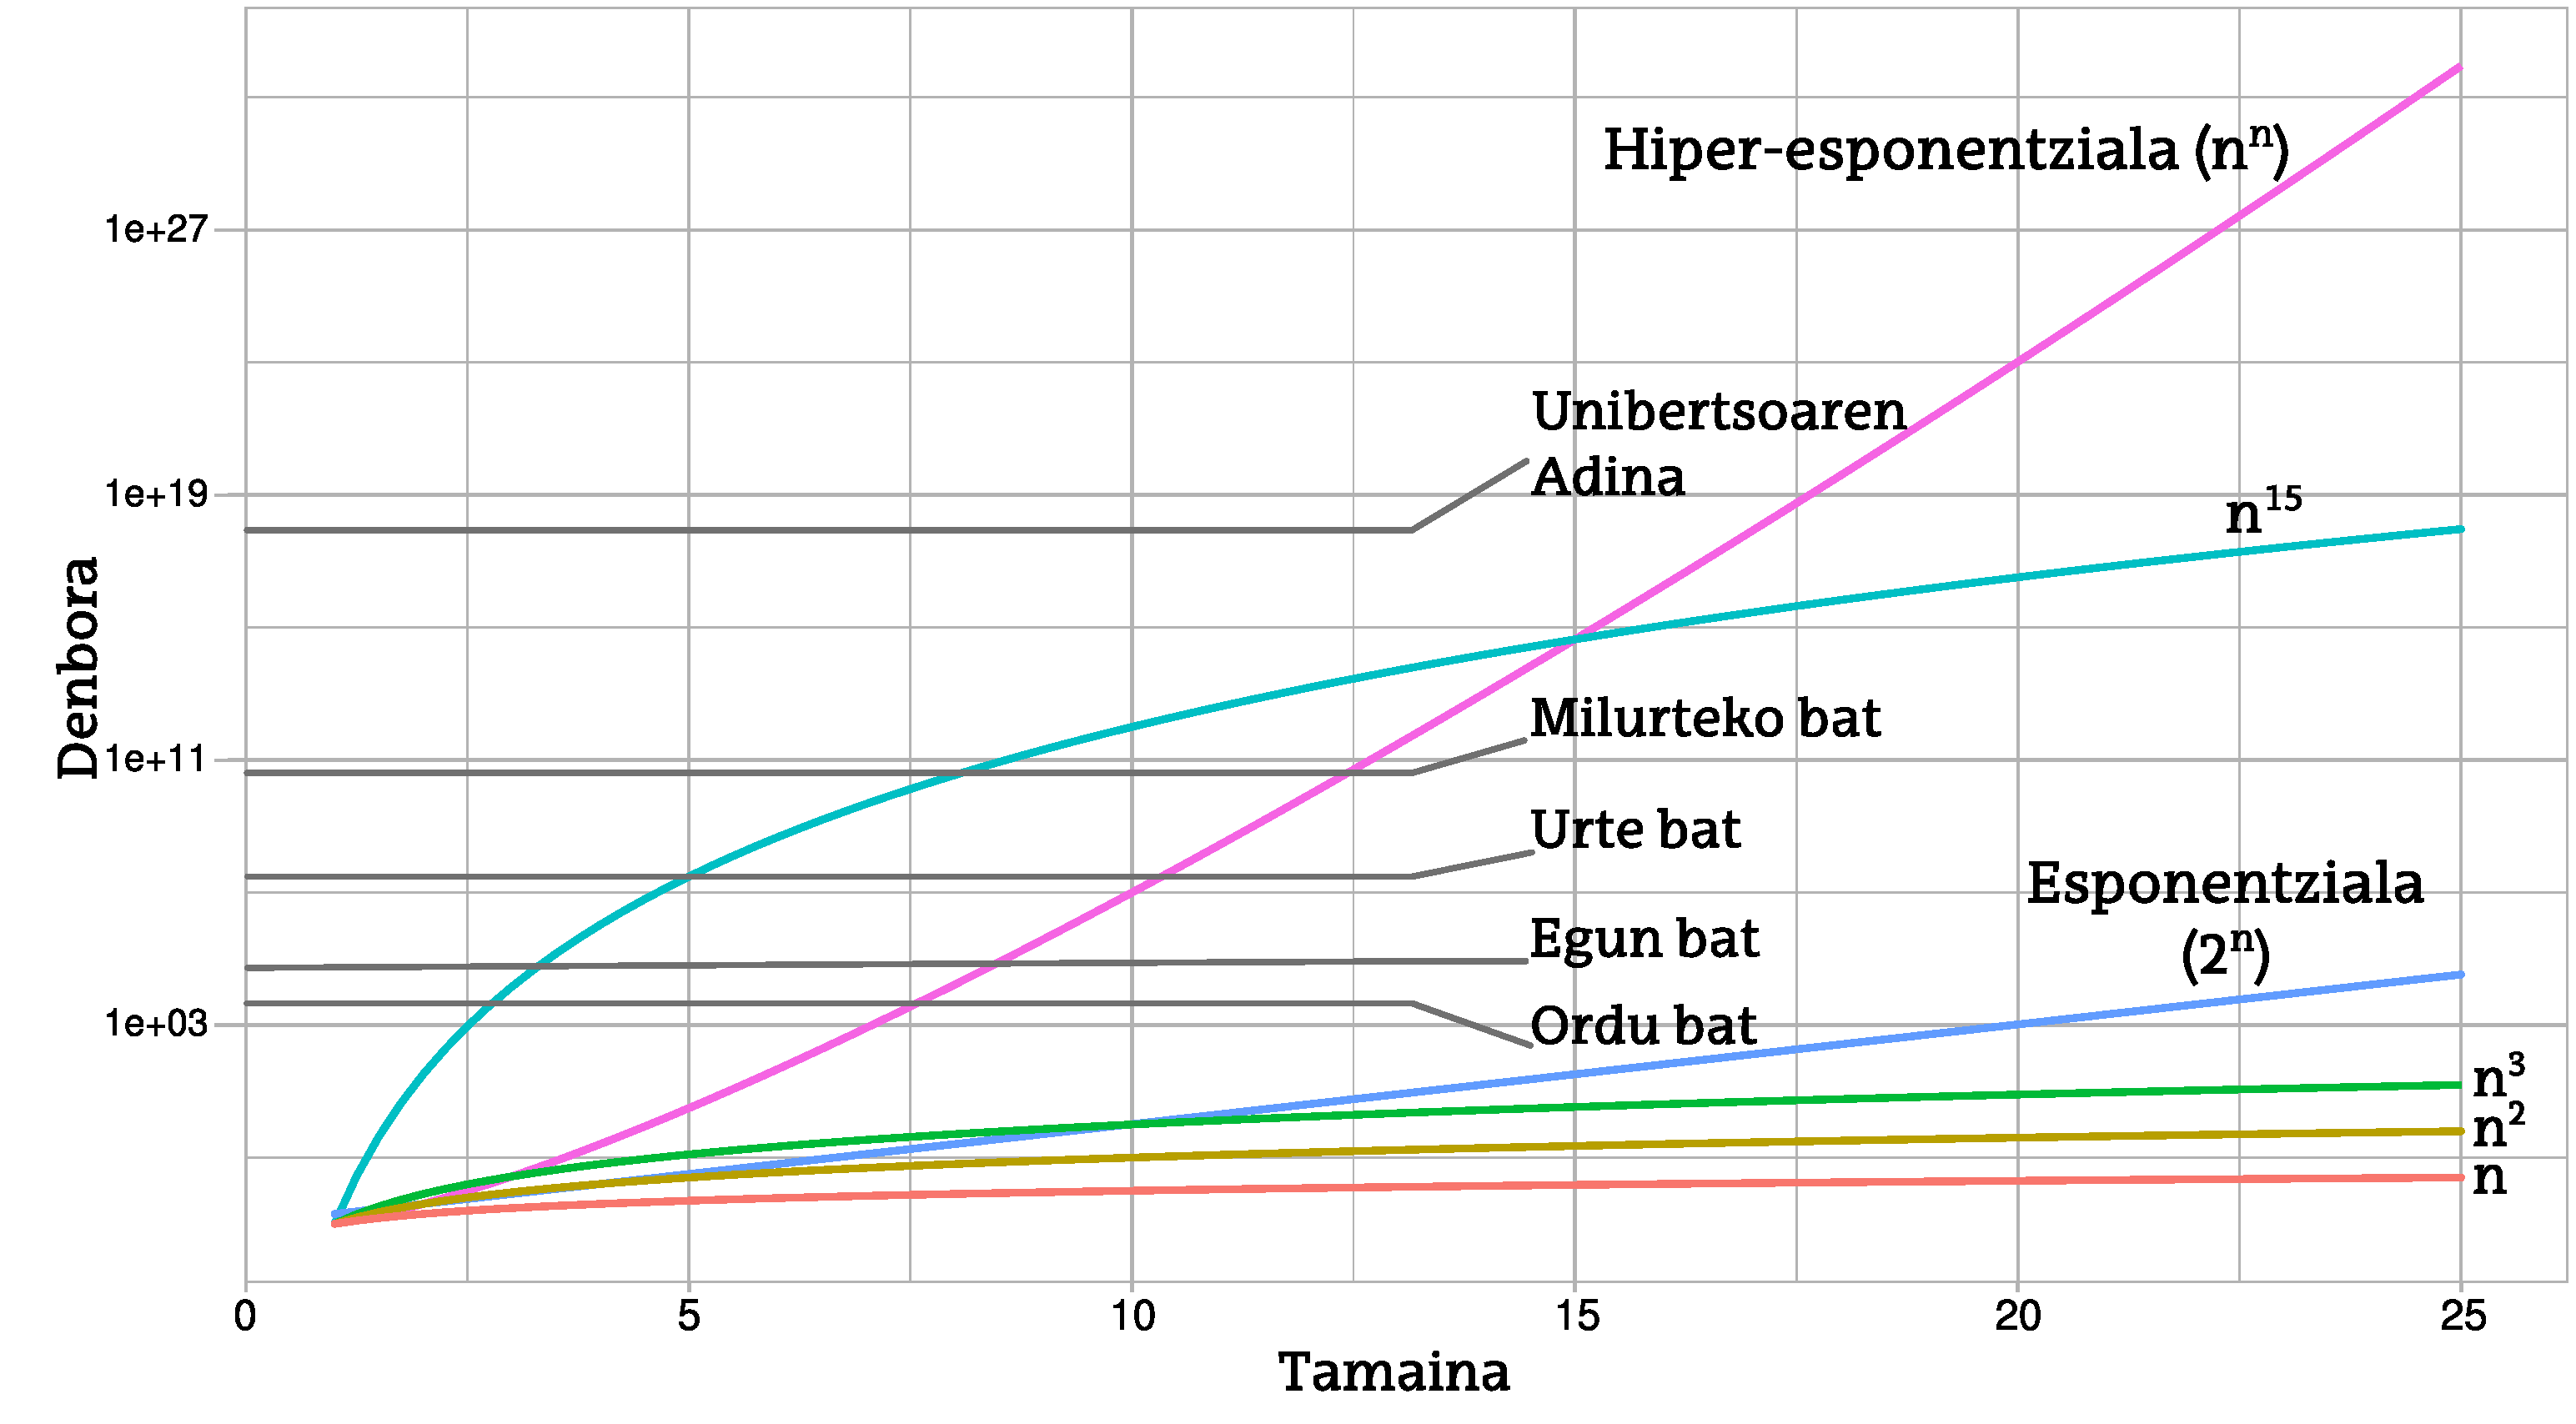
\includegraphics[width=\linewidth]{./Irudiak/complexity_orders}
\caption{Konplexutasun ordena tipikoen hazkunde abiadura $n$-rekiko.}
\label{fig:complexity_orders}
\end{figure}

\subsection{Problema klasikoak}

Errealitatean ebatzi behar izaten diren optimizazio problema guztiak ezberdinak dira, kasu bakoitzak bere murrizketa edota baldintza bereziak baititu. Diferentziak diferentzia, problema askoren mamia bertsua da; hala nola, garraio-problemak, esleipen-problemak, antolakuntza-problemak, etab. Hori dela eta, optimizazioaren arloan askotan problema teorikoak aztertzea izaten da ohikoena, errealitatean topa ditzakegun problemen abstrakzioak edota sinplifikazioak direlarik. Atal honetan optimizazio problema teoriko klasiko batzuk aztertuko ditugu. % --XXX eranskinean problema gehiago topa ditzakezu--.

\subsubsection{Garraio-problemak}\label{sec:tsp}

Merkantziak edota pertsonen garraioarekin zerikusia duten optimizazio problemak Ikerkuntza Operatiboan aztertu izan diren problemetatik lehenetarikoak dira. Oinarrizko garraio-probleman iturburu-puntuak eta helburu-puntuak ditugu; halaber, iturburu-puntu bakoitzetik helburu-puntu bakoitzera elementuen garraio kostua dugu, kostu matrizean jasota. Iturburu-puntu bakoitzaren eskaintza eta helburu-puntu bakoitzaren eskaera ezagunak dira. Problemaren helburua eskaera guztiak asetzeko kostu minimoko garraio-eskema topatzea da, iturburu-puntuek dituen mugak (eskaintzak) gainditu barik. 

Problema sinple hau eredu linealen bidez modela daiteke eta, hortaz, badaude algoritmo eraginkorrak ebazteko. Alabaina, badaude garraioari buruzko beste hainbat problema klasiko NP direnak. Ezagunena, \textit{Travelling Salesman Problem}-a~\cite{goldberg1985} da --hau da, Saltzaile Bidaiariaren Problema--. 

\begin{tcolorbox}
\begin{ifexample}{\bf Saltzaile Bidaiariaren Problema (Travelling Salesman Problem, TSP)}
Demagun saltzaile bidaiariak garela eta egunero hainbat bezero bisitatu behar ditugula. Bezero bakoitza herri batean bizi da eta, edozein bi herrien arteko distantzia ezaguna izanda, gure helburua herri guztietatik pasatzen den ibilbiderik motzena topatzea da.
\end{ifexample}
\end{tcolorbox}

\begin{figure}[t]
\centering
\subfigure[Mapa]{
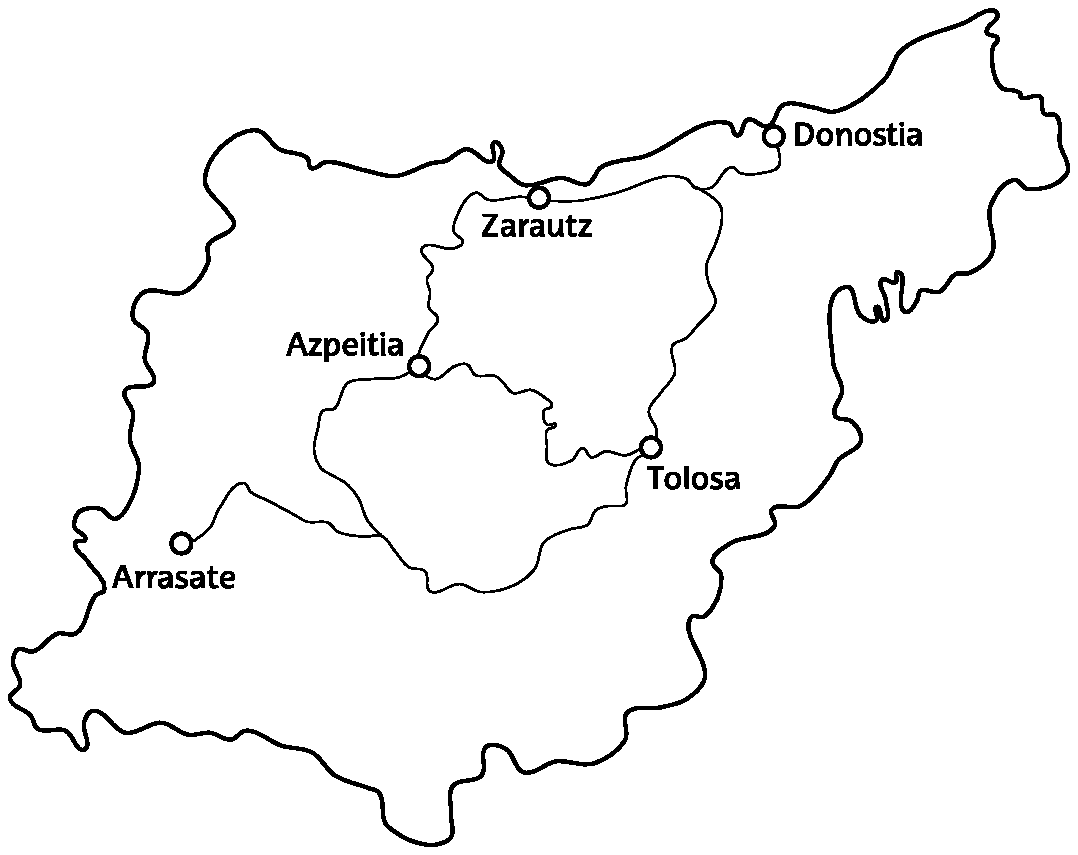
\includegraphics[width=0.45\linewidth]{./Irudiak/mapa}}
\subfigure[Dagokion grafoa]{
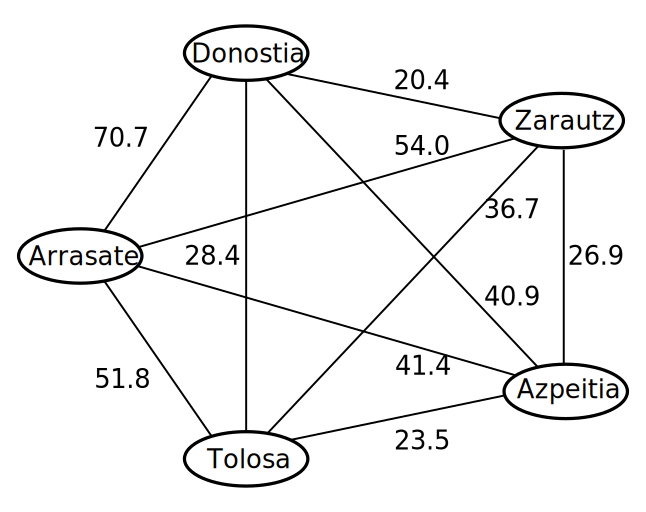
\includegraphics[width=0.45\linewidth]{./Irudiak/grafo_TSP}}
\caption{TSP-aren adibide bat, bost herriekin}
\label{fig:tsp}
\end{figure}

Problema honen hastapenak Irlandan daude, Hamilton matematikariaren lanetan. Problema formalizatzeko grafo oso bat eraiki dezakegu non erpinak herriak diren eta edozein bi erpinen artean ertz pisudun bat daukagun; ertzen pisua, lotzen dituen bi herrien arteko distantzia da (ikusi \ref{fig:tsp} irudiak). Horrela ikusita, herri bakoitzetik bakarrik behin igaro nahi badugu, problemaren soluzioak ziklo Hamiltoniarrak izango dira --hots, zikloak zeinentzat nodo guztiak behin eta bakarrik behin agertzen diren--. Ziklo Hamiltoniar guztien artean pisu totala minimoa duena bilatu nahi dugu. 

Arrasate, Zarautz, Tolosa, Azpeitia, Donostia ibilbidea, irudian agertzen den problemarako soluzio bat; soluzio honen ebaluazioa ondorengoa izango da:

\begin{itemize}
\item Arrasate - Zarautz: 54.0
\item Zarautz - Tolosa: 36.7
\item Tolosa - Azpeitia: 23.5
\item Azpeitia - Donostia: 40.9
\item Donostia - Arrasate: 70.7
\end{itemize}

Hortaz, helburu funtzioa --ibilbidearen distantzia totala, alegia-- 225.8 da. Ikus dezagun adibidea R-n. Lehenik eta behin, \code{metahuR} paketea kargatu eta problemaren helburu funtzioa sortuko dugu:

\begin{knitrout}
\definecolor{shadecolor}{rgb}{1, 1, 1}\color{fgcolor}\begin{kframe}
\begin{alltt}
\hlstd{> }\hlkwd{library}\hlstd{(}\hlstr{"metaheuR"}\hlstd{)}
\hlstd{> }\hlstd{cost.matrix} \hlkwb{<-} \hlkwd{matrix}\hlstd{(}\hlkwd{c}\hlstd{(}\hlnum{0} \hlstd{,} \hlnum{20.4} \hlstd{,} \hlnum{40.9} \hlstd{,} \hlnum{28.4} \hlstd{,} \hlnum{70.7} \hlstd{,}
\hlstd{+ }                        \hlnum{20.4} \hlstd{,} \hlnum{0} \hlstd{,} \hlnum{26.9} \hlstd{,} \hlnum{36.7} \hlstd{,} \hlnum{54} \hlstd{,}
\hlstd{+ }                        \hlnum{40.9} \hlstd{,} \hlnum{26.9} \hlstd{,} \hlnum{0} \hlstd{,} \hlnum{23.5} \hlstd{,} \hlnum{41.4} \hlstd{,}
\hlstd{+ }                        \hlnum{28.4} \hlstd{,} \hlnum{36.7} \hlstd{,} \hlnum{23.5} \hlstd{,} \hlnum{0} \hlstd{,} \hlnum{51.8} \hlstd{,}
\hlstd{+ }                        \hlnum{70.7} \hlstd{,} \hlnum{54} \hlstd{,} \hlnum{41.4} \hlstd{,} \hlnum{51.8} \hlstd{,} \hlnum{0}\hlstd{) ,} \hlkwc{nrow}\hlstd{=}\hlnum{5}\hlstd{)}
\hlstd{> }\hlstd{city.names} \hlkwb{<-} \hlkwd{c}\hlstd{(}\hlstr{"Donostia"}\hlstd{,}\hlstr{"Zarautz"}\hlstd{,}\hlstr{"Azpeitia"}\hlstd{,}\hlstr{"Tolosa"}\hlstd{,}\hlstr{"Arrasate"}\hlstd{)}
\hlstd{> }\hlkwd{colnames}\hlstd{(cost.matrix)} \hlkwb{<-} \hlstd{city.names}
\hlstd{> }\hlkwd{rownames}\hlstd{(cost.matrix)} \hlkwb{<-} \hlstd{city.names}
\hlstd{> }\hlstd{cost.matrix}
\end{alltt}
\begin{verbatim}
##          Donostia Zarautz Azpeitia Tolosa Arrasate
## Donostia      0.0    20.4     40.9   28.4     70.7
## Zarautz      20.4     0.0     26.9   36.7     54.0
## Azpeitia     40.9    26.9      0.0   23.5     41.4
## Tolosa       28.4    36.7     23.5    0.0     51.8
## Arrasate     70.7    54.0     41.4   51.8      0.0
\end{verbatim}
\begin{alltt}
\hlstd{> }\hlstd{tsp.example} \hlkwb{<-} \hlkwd{tsp.problem}\hlstd{(}\hlkwc{cmatrix} \hlstd{= cost.matrix)}
\end{alltt}
\end{kframe}
\end{knitrout}

Orain, lehen aipatutako soluzioa sortu eta ebaluatu egingo dugu.

\begin{knitrout}
\definecolor{shadecolor}{rgb}{1, 1, 1}\color{fgcolor}\begin{kframe}
\begin{alltt}
\hlstd{> }\hlstd{solution} \hlkwb{<-} \hlkwd{permutation}\hlstd{(}\hlkwd{c}\hlstd{(}\hlnum{5}\hlstd{,}\hlnum{2}\hlstd{,}\hlnum{4}\hlstd{,}\hlnum{3}\hlstd{,}\hlnum{1}\hlstd{))}
\hlstd{> }\hlstd{tsp.example}\hlopt{$}\hlkwd{evaluate} \hlstd{(solution)}
\end{alltt}
\begin{verbatim}
## [1] 225.8
\end{verbatim}
\end{kframe}
\end{knitrout}

Hona hemen pentsatzeko galdera batzuk:
\begin{itemize}
  \item Distantzia totala 225.8km-koa da baina, ba al da ibilbide hau distantzia minimokoa?.  
  \item Proba ezazu, adibidez, Azpeitia eta Tolosa trukatzen. Soluzio berri hau hobea ala okerragoa da?. 
  \item Zenbat ibilbide daude bost herri hauek behin eta bakarrik behin bisitatzen dutenak?
\end{itemize}

\begin{ifproblem}
Inplementa ezazu funtzio bat \code{n} tamainako TSP problema bat eta bere ebaluazio funtzioa emanda, soluzio guztiak ebaluatzen dituena bide motzena topatzeko.
\end{ifproblem}

Ikus dezagun nola formaliza daitekeen TSP problema matematikoki:

\begin{ifdefinition}{\bf TSP problema} -
Izan bedi $H={h_1, \ldots, h_n}$ kokapen zerrenda eta $A\in\mathbb{R}^{n\times n}$ distantzia matrizea non $a_{ij}$, $h_i$ eta $h_j$ kokapenen artean dagoen distantzia den. TSP problema ibilbide optimoa topatzean datza, hau da, kokapen guztietatik behin eta bakarrik behin igarotzen diren ibilbideetatik motzena.
\end{ifdefinition}

TSP-aren definizioan kostu matrizea simetrikoa dela suposatzen da. Hala ere, kasu errealetan, posible da norabide batean istripu bat egotea edo bidea noranzko batean eta bestean ezberdinak izatea. Egoera hauetan biden kostuak simetrikoak direla suposatzea ez da problema modelatzeko aukerarik logikoena. Hortaz, bi TSP problema mota defini daitezke: simetrikoa eta asimetrikoa. 

TSP-a oso erabilia da algoritmoak probatzean, eta TSPLIB liburutegian~\cite{reinelt1990} hainbat instantzia eskuragarri daude, orain arte lortutako soluziorik onenen informazioarekin batera.

\subsubsection{Esleipen-problemak}

Matematikako eta, batez ere, Ikerkuntza Operatiboko oinarrizko problemak dira. Esleipen-problemetan aldaera konbinatorio asko aurkitu ditzakegun arren, funtsean denak ondorengo ideian oinarritzen dira:

Demagun $n$ agente ditugula, $m$ ataza burutzeko. Agente bakoitzak kostu konkretu bat du ataza bakoitza burutzeko eta ataza bakoitza betetzeaz agente bakar bat arduratu behar da.  Esleipen-problemaren helburua, ataza bakoitzari agente bat esleitzean datza, ataza guztiak burutzeko kostu totala minimizatuz.

Problema honen kasu nabariena Esleipen Problema Lineala da --\textit{Linear Assignment Problem}, ingelesez--, non agente eta ataza kopurua berdina den, eta esleipen kostu totala eta agente bakoitzaren kostuen batura totala ere berdinak diren. 1955ean Harold Kuhn-ek Algoritmo Hungariarra proposatu zuen, zeinek Esleipen Problema Lienala denbora polinomialean ($O(n^4)$) ebazten duena, $n$ agente kopurua izanik. Badago ordea, esleipen problema mota bat, NP-zaila dena eta liburuan adibide gisa erabiliko duguna: Esleipen Problema Koadratikoa --\textit{Quadratic Assignment Problem}, QAP,~\cite{burkard1998} ingelesez--.

\begin{ifdefinition} {\bf QAP Problema} Izan bitez $n$ instalazio, $n$ kokapen posible, $H\in\mathbb{R}^{n\times n}$ instalazioen arteko fluxu matrizea, eta $D\in\mathbb{R}^{n\times n}$ kokapenen arteko distantzia matrizea. QAP problemaren helburua, instalazio bakoitza kokapen batean finkatzean datza, kostu totala minimizatuz
\end{ifdefinition}


\subsubsection{Antolakuntza-problemak}

Prozesu, lan edota ataza desberdinen antolakuntza eta zerbitzatzearekin zerikusia duten optimizazio problemak dira. Antolakuntza-problemen helburua kudeatzaileak jasotzen dituen lan eskariak, modurik eraginkorrenean zerbitzatzea da. Eraginkortasunaren neurria, problemaren araberakoa da; hala ere, eskariak ahalik eta denbora/kostu txikienean asetzea da irizpide ohikoena.

Hasiera batean, antolakuntza-problema gehientsuenak industriarekin zerikusia zuten domeinuetan proposatu ziren. Produktuaren ekoizpenerako makineria erabiltzen zen enpresetan, etekina maximizatzea zen helburua, makineriaren eta baliabideen erabilera, mantentze-kostuak, etab. optimizatuz. Aldi berean, langileen ordutegien planifikazioan antzerako ezaugarriak zituen problemak ere proposatu ziren.

Gaur egun ordea, problema hauek edozein arlotara daude hedatuta. Esate baterako, konputazioan, konputagailuen Prozesurako Unitate Zentralak (PUZ), \textit{scheduler} eta \textit{dispatcher} izeneko tresnak erabiltzen ditu, jasotzen dituen prozesuak erarik eraginkorrenean zerbitzatzeko, denbora eta memoriaren erabilera minimizatuz.

Adibide gisa, jarraian, antolakuntza problemetan oso ezaguna den Muntaketa-kateko Plangintza-Problema --\textit{Permutation Flowshop Scheduling Problem}, PFSP ~\cite{gupta2006} ingelesez-- aztertuko dugu:

\begin{ifdefinition} {\bf PFSP problema}. Izan bitez, $n$ lan, $m$ makina eta $P\in\mathbb{R}^{n\times m}$ prozesamendu denboren matrizea, non $p_{ij}$ elementuan $i$ eta $j$ lanaren eta makinaren identifikadoreak diren, hurrenez hurren. Lan bakoitza burutzeko, $m$ prozesu desberdin aplikatu behar dira, bakoitza makina batean, hau da, $j$-garren operazioa, $j$-garren makinan egingo da. Behin $i$ lana $j$ makinan sartzen denean prozesatzeko, eten barik prozesatuko da, eta denbora konkretu bat emango du bertan, $p_{ij}$. $i$ lana $j$ makinatik irten denean, $j+1$ makinara pasako da hurrengo prozesua burutzera, baldin eta makina hau libre badago. PFSPa lanak prozesatzeko denbora totala minimizatzen duen $n$ lanen sekuentzia optimoa aurkitzean datza.
\end{ifdefinition}

\begin{figure}[t]
\centering
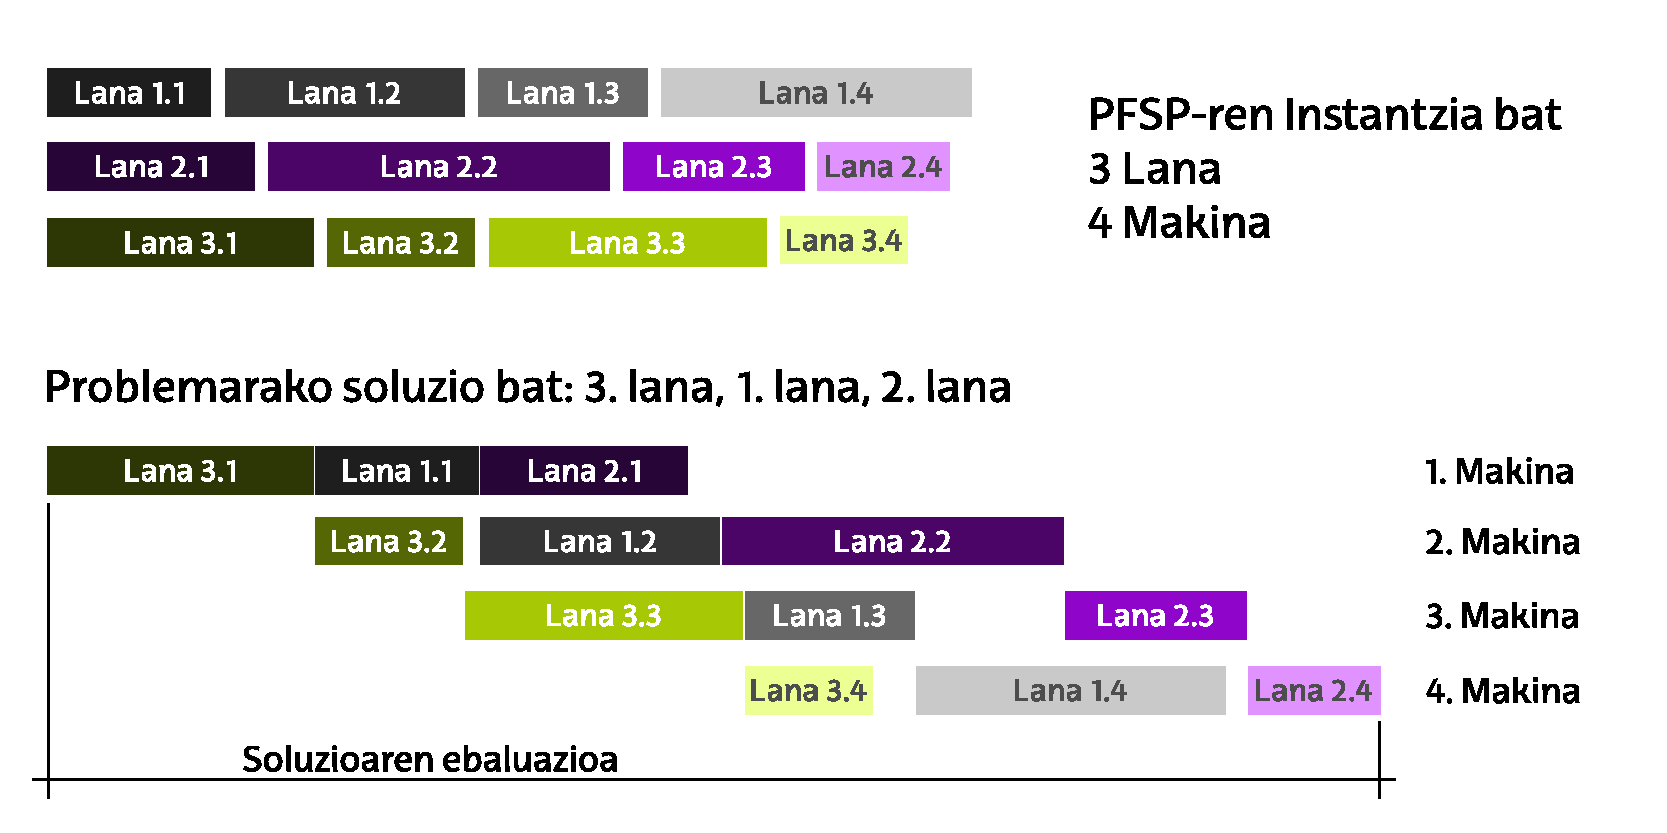
\includegraphics[width=0.75\linewidth]{./Irudiak/PFSP}
\caption{PFSP problemaren adibide bat. Goiko partean problemaren definizioa dago, hau da, lan bakoitza burutzeko makina bakoitzean behar den denbora. Beheko partean soluzio bat eta bere interpretazioa erakusten da. Helburua denbora totala minimizatzea bada, lana 3.1 hasten denetik lana 2.4 amaitzen den arte igarotzen duen denbora da soluzioaren ebaluazioa}
\label{fig:pfsp}
\end{figure}

\ref{fig:pfsp} irudian problemaren instantzia bat ikus daiteke. Adibide honetan 3 lan egin behar dira, 4 makina ezberdinetan prozesatuz. Irudiaren goiko partean lan bakoitzak makina bakoitzean igaro behar duen denbora adierazten da, lauki zuzenen bidez. Irudiaren beheko partean soluzio bat proposatzen da; lanak 3,1,2 ordenean prozesatuko dira. Honek esan nahi du 3. lana 1. makinan sartuko dela. Behar duen denbora pasatzen denean, 2. makinan sartuko da eta 1. makinan 1. lana sartuko da. Prozesu guztiaren eskema irudian ikus daiteke. Problemaren helburua denbora total minimizatzea bada, soluzio honen helburu funtzioaren balioa lana 3.1 hasten denetik Lana 2.4 amaitzen den arte igarotzen duen denbora izango da.


PFSP, antolakuntza problemen murriztapenik gabeko problema teorikoa da. Problema errealetan, lan kopurua ez da finitua, etengabekoa baizik; kasu horietan, makinen okupazio maila altua izatea, denbora murriztea bezain garrantzitsua izaten da. Zentzu honetan, antzeko problemen aukera oso zabala da~\cite{taillard1993}.

\subsubsection{Azpimultzo-problemak}\label{sec:subset_problems}

Demagun objektu multzo bat dugula, eta multzo honetatik, objektu batzuk aukeratu behar ditugula. Aukeraketa, ez da ausaz egingo, baizik eta irizpide eta murriztapen batzuei jarraituz. Azpimultzo-problematan, helburua aukeraketak ematen dizkigun onurak maximizatzean datza, definitutako murriztapenak betetzen direlarik.

Azpimultzo-problemen hedapena oso zabala da, logistikako alorretan, gehien bat: kargarako garraiobideen betetzea, aurrekontuaren kontrola, finantzen kudeaketa, industriako materialen ebaketa, etab.

Azpimultzo-problemen artean adibide erakusgarriena -- eta bidenabar sinplifikagarriena -- ingelesez \textit{0-1 Knapsack problem} deritzon 0-1 Motxilaren problema~\cite{kellerer2004} da. Jarraian zehazki azalduko dugu problema hau:

\begin{ifdefinition} {\bf 0-1 Motxilaren Problema}. Izan bitez $n$ objektu, $c$ motxilaren edukiera maximoa, eta $P\in\mathbb{R}^n$ eta $W\in\mathbb{R}^n$ objektuen balio- eta pisu-bektoreak hurrenez hurren. Problema honetan, $n$ objektuen artetik aukeratzen ditugun elementuen balio totala maximizatzea dugu helburu, motxilaren edukiera maximoa gainditu gabe betiere. 
\end{ifdefinition}


\subsubsection{Grafoei buruzko problemak}
Grafoak, matematika eta informatikan funtsezko egiturak dira. Orokorrean grafoak objektuen arteko erlazioak adierazteko erabiltzen dira eta, beraz, beraien erabilera edozein domeinutan da aplikagarria. Hori dela eta, grafoei loturiko problemen multzoa oso zabala da. Esaterako, berriki ikusi ditugun TSP eta QAP-ak grafo problema gisa formaliza ditzakegu. Garraiobide eta esleipen problemez gain, sareko informazio trukaketa edota grafoen teoriako problema ugari (deskonposizio-problemak, azpimultzo-problemak, estaldura-problemak, etc.) ebazteko erabili ohi dira.

Atal honetan, ingelesez \textit{Graph Coloring} deritzon Grafoen Koloreztatze-Problema izango dugu aztergai.

\begin{ifdefinition} {\bf Grafoen Koloreztatze-Problema}. Izan bedi $G=(V,E)$ grafoa non $V$ eta $E$ bektoreak grafoaren erpin- eta ertz-multzoak diren, hurrenez hurren; $e_{ij}\in E$ existitzen bada $v_i$ eta $v_j$ erpinen artean ertza dago. Erpin bakoitzari kolore bat esleitu behar diogu, kontuan hartuz $e_{ij}\in E$ existitzen bada, $v_i$ eta $v_j$ nodoek ezin dutela kolore bera izan; hau da, ertz baten bidez lotutako erpinak kolore ezberdinekin koloreztatu behar dira. Problemaren helburua kolore kopuru minimoa erabiltzen duen koloreztatzea topatzean datza.
\end{ifdefinition}

Ikus dezagun adibide pare bat, ausaz sortutako grafo bat erabiliz. Jarraian dagoen kodean 15 erpin dituen ausazko grafo bat sortu ondoren, koloreztatze-problema bat sortuko dugu, \code{metaheuR} paketean dagoen funtzioak erabiliz.

\begin{knitrout}
\definecolor{shadecolor}{rgb}{1, 1, 1}\color{fgcolor}\begin{kframe}
\begin{alltt}
\hlstd{> }\hlkwd{library}\hlstd{(}\hlstr{"igraph"}\hlstd{)}
\hlstd{> }\hlkwd{set.seed}\hlstd{(}\hlnum{1623}\hlstd{)}
\hlstd{> }\hlstd{n} \hlkwb{<-} \hlnum{15}
\hlstd{> }\hlstd{rnd.graph} \hlkwb{<-} \hlkwd{random.graph.game}\hlstd{(n ,} \hlkwc{p.or.m} \hlstd{=} \hlnum{0.2}\hlstd{)}
\hlstd{> }\hlstd{gcol.problem} \hlkwb{<-} \hlkwd{graph.coloring.problem} \hlstd{(rnd.graph)}
\end{alltt}
\end{kframe}
\end{knitrout}

Ausazko soluzio bat sortzen dugu, bakarrik 3 kolore erabiliz. Kontutan hartu behar da soluzioa \code{factor} motako bektore bat izan behar dela, non balio posibleen kopurua nodoen kopuru berdina izan behar den (kasurik txarrenean, grafo osoa denean, nodo bakoitzak kolore ezberdin bat izan beharko du). Ausazko soluzioa ea bideragarria denetz egiaztatuko dugu, problema definitzean \code{is.valid} sortutako funtzioa erabiliz.

\begin{knitrout}
\definecolor{shadecolor}{rgb}{1, 1, 1}\color{fgcolor}\begin{kframe}
\begin{alltt}
\hlstd{> }\hlstd{rnd.sol} \hlkwb{<-} \hlkwd{factor} \hlstd{(}\hlkwd{paste}\hlstd{(}\hlstr{"c"}\hlstd{,}\hlkwd{sample}\hlstd{(}\hlnum{1}\hlopt{:}\hlnum{3} \hlstd{,} \hlkwc{size} \hlstd{= n ,} \hlkwc{replace} \hlstd{= T) ,} \hlkwc{sep}\hlstd{=}\hlstr{""}\hlstd{) ,}
\hlstd{+ }                   \hlkwc{levels} \hlstd{=} \hlkwd{paste}\hlstd{(}\hlstr{"c"} \hlstd{,} \hlnum{1}\hlopt{:}\hlstd{n ,} \hlkwc{sep}\hlstd{=}\hlstr{""}\hlstd{))}
\hlstd{> }\hlstd{rnd.sol}
\end{alltt}
\begin{verbatim}
##  [1] c1 c1 c1 c3 c1 c2 c2 c1 c1 c3 c2 c1 c1 c2 c2
## Levels: c1 c2 c3 c4 c5 c6 c7 c8 c9 c10 c11 c12 c13 c14 c15
\end{verbatim}
\begin{alltt}
\hlstd{> }\hlstd{gcol.problem}\hlopt{$}\hlkwd{is.valid}\hlstd{(rnd.sol)}
\end{alltt}
\begin{verbatim}
## [1] FALSE
\end{verbatim}
\begin{alltt}
\hlstd{> }\hlstd{gcol.problem}\hlopt{$}\hlkwd{plot}\hlstd{(rnd.sol ,} \hlkwc{node.size} \hlstd{=} \hlnum{15} \hlstd{,} \hlkwc{label.cex} \hlstd{=} \hlnum{1.5}\hlstd{)}
\end{alltt}
\end{kframe}
\end{knitrout}

\begin{figure}[t]
\subfigure[Soluzio bideraezina]{
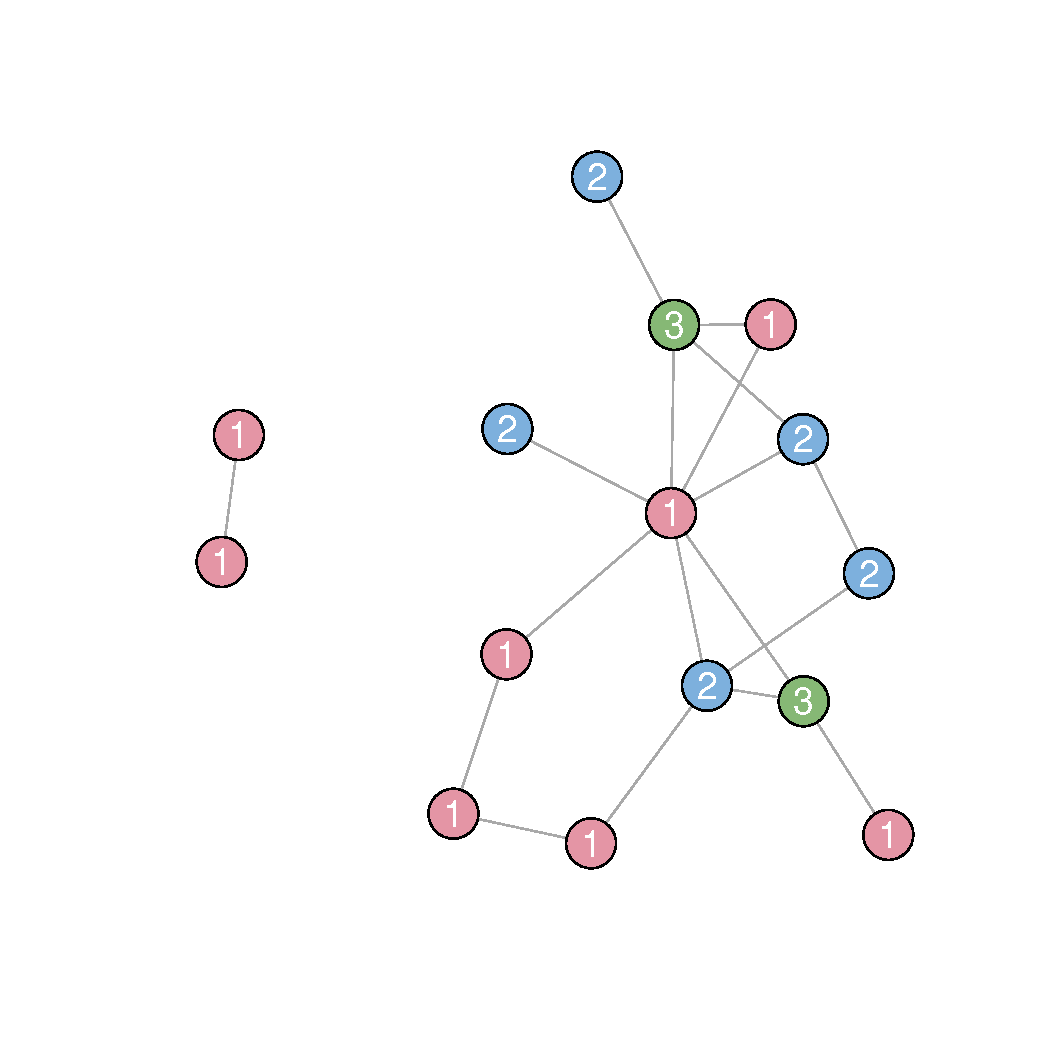
\includegraphics[width=0.45\textwidth] {./Irudiak/Graph_coloring_2_-1}
}
\subfigure[Soluzio bideragarria]{

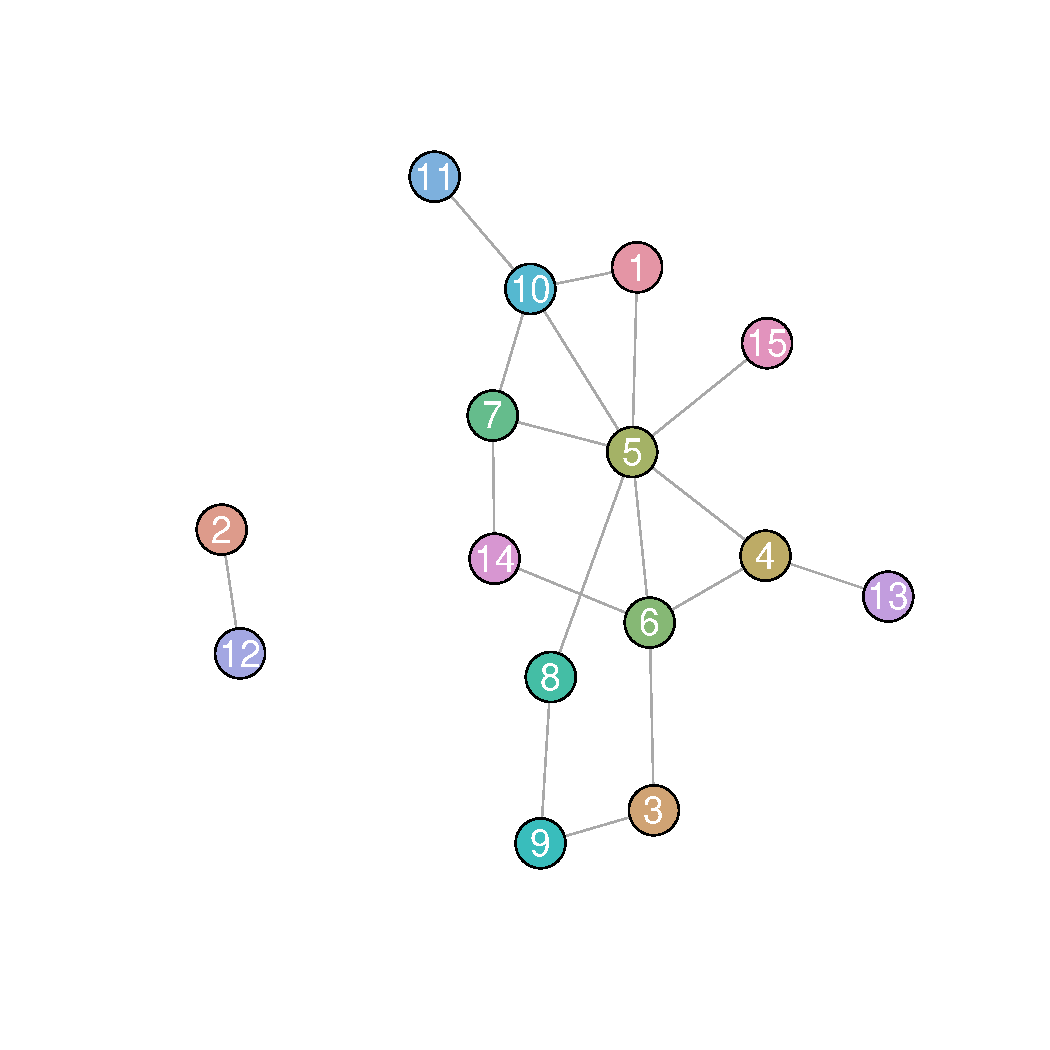
\includegraphics[width=0.45\textwidth] {./Irudiak/Graph_coloring_3_-1}
}
\caption{Grafoen koloreztatze-problemaren bi adibide. Lehenengoa, (a), bideraezina da, elkar ondoan dauden nodo batzuk kolore berdina baitute. Bigarrena, (b), soluzio bideragarri tribiala da, nodo bakoitzak kolore ezberdin bat baitu.}\label{fig:graph_coloring}
\end{figure}

Soluzioa bideraezina da, \ref{fig:graph_coloring} (a) irudian ikus daitekeen legez. Soluzio bideragarri bat sortzeko era sinple bat badago: nodo bakoitzari kolore ezberdin bat esleitu (ikusi \ref{fig:graph_coloring} (b) irudia).

\begin{knitrout}
\definecolor{shadecolor}{rgb}{1, 1, 1}\color{fgcolor}\begin{kframe}
\begin{alltt}
\hlstd{> }\hlstd{trivial.sol} \hlkwb{<-} \hlkwd{factor} \hlstd{(}\hlkwd{paste}\hlstd{(}\hlstr{"c"} \hlstd{,} \hlnum{1}\hlopt{:}\hlstd{n ,} \hlkwc{sep}\hlstd{=}\hlstr{""}\hlstd{) ,}
\hlstd{+ }                   \hlkwc{levels} \hlstd{=} \hlkwd{paste}\hlstd{(}\hlstr{"c"} \hlstd{,} \hlnum{1}\hlopt{:}\hlstd{n ,} \hlkwc{sep}\hlstd{=}\hlstr{""}\hlstd{))}
\hlstd{> }\hlstd{trivial.sol}
\end{alltt}
\begin{verbatim}
##  [1] c1  c2  c3  c4  c5  c6  c7  c8  c9  c10 c11 c12 c13 c14 c15
## Levels: c1 c2 c3 c4 c5 c6 c7 c8 c9 c10 c11 c12 c13 c14 c15
\end{verbatim}
\begin{alltt}
\hlstd{> }\hlstd{gcol.problem}\hlopt{$}\hlkwd{is.valid}\hlstd{(trivial.sol)}
\end{alltt}
\begin{verbatim}
## [1] TRUE
\end{verbatim}
\begin{alltt}
\hlstd{> }\hlstd{gcol.problem}\hlopt{$}\hlkwd{plot}\hlstd{(trivial.sol ,} \hlkwc{node.size} \hlstd{=} \hlnum{15} \hlstd{,} \hlkwc{label.cex} \hlstd{=} \hlnum{1.5}\hlstd{)}
\end{alltt}
\end{kframe}
\end{knitrout}


\subsubsection{Karaktere-kate problemak}
Optimizazio konbinatorioko karaktere-kateen arteko erlazioak aurkitzeaz arduratzen diren problemen multzoa da. Problema ezagunenetariko bat Azpisekuentzia Komun Luzeenaren Problema --Longest Common Subsequce Problem, LCSP-- da. Izenak berak adierazten duen bezala, ditugun karaktere-kateen edo sekuentzien artean komuna den azpisekuentzia luzeena bilatzen duen problema da\footnote{Kontutan hartu azpisekuentzia eta karaktere azpi-kate kontzeptuak ezberdinak direla, bigarrenean hautatutako elementuak jarraian egon behar baitira jatorrizko sekuentzian baina lehenengoan ez. Hau da, $CTTTCGTCATA$ sekuentzia badugu, $TCGTCA$ bai azpisekuentzia eta baita azpi-katea ere bada, baina $GTA$ azpisekuentzia izan arren ez da azpi-katea}.

\begin{tcolorbox}
\begin{ifexample}
Demagun hiru DNA sekuentzia ditugula; CACGACGCGT, CGTTTCGCAG eta CTTGCGCGA. Hiru sekuentzietan dagoen azpisekuentzia komun luzeena CGCGCG da; hau da, caCGaCGCGt, CGtttCGCaG, eta CttGCGCGa daukagu. Beste edozein letra sartuz gero, azpisekuentzia ez da sarrerako hiru sekuentzietan agertuko.
\end{ifexample}
\end{tcolorbox}

LCSP-a formalizatzeko lehendabizi azpisekuentzia kontzeptua definitu behar dugu.

\begin{ifdefinition}
Izan bedi $\Sigma$ alfabetoan definitutako $n$ tamainako sekuentzia $S=(s_1,\ldots,s_n)$, hau da, $\forall i=1,\ldots,n$, $s_i\in \Sigma$. $S^\prime=(s_{a_1},\ldots,s_{a_m})$ $S$-ren azpisekuentzia da baldin eta soilik baldin $a_i\in\{1,\ldots,n\}$ eta $\forall j=2\ldots,m$, $a_{i-1}<a_i$
\end{ifdefinition}

Hau da, azpisekuentzia batean jatorrizko sekuentzian dauden elementuen azpimultzo bat izango dugu, \textit{jatorrizko sekuentzian agertzen diren ordena berdinarekin}. Sekuentzia bat emanda, bere zenbait elementu ezabatuz lor ditzakegu azpisekuentziak.

Bi sekuentzia besterik ez badugu --$m$ eta $n$ tamainakoak-- LCSP-a programazio dinamikoa erabiliz\footnote{Problema hau sekuentziak lerrokatzean agertzen da; kasu honetan, nahiz eta algoritmo polinomikoa izan, sekuentziak milioika elementu izan dezaketenez, programazio dinamikoaz gain metodo heuristikoak erabiltzen dira; metodorik ezagunena BLAST\citep{altschul1990} izenekoa da} $O(mn)$ denboran ebatz daiteke; sekuentzia kopurua finkaturik gabe badago, ordea, problema NP-zaila da.

\begin{ifdefinition}{\bf Longest Common Subsequence Problema (LCSP)}
Izan bitez $\Sigma$ alfabetoan definitutako tamaina ezberdineko $k$ sekuentzia $S_1,\ldots,S_k$. Izan bedi $k$ sekuentzien azpisekuentzia diren sekuentzia multzoa $\cal C$. LCSP-aren helburua $C^*\in{\cal C}$ sekuentzia topatzea da, non $\forall C_i\in{\cal C}\ |C_i|>|C^*|$.
\end{ifdefinition}

LCSP bezalako problemak ohikoak izaten dira terminaleko komandoetan, adibidez, \texttt{diff} edo \texttt{grep} komandoetan.

Azken hamarkadetan ordea, Bioinformatika arloak lortu duen arretarekin, karaktere-kate problema ugari proposatu dira. Horietako bat, Sekuentzia-zati Muntaketa Problema -- \textit{Fragment Assembly Problem}, FAP, ingelesez-- da. DNA-ren sekuentziaziorako teknologia ez dago hain aurreratua, eta gaur egun oraindik ezinezkoa da genomen karaktere-kateak osorik irakurtzea. Hori dela eta, DNA zatitxoak irakurtzea ahalbidetzen duen bestelako teknikak erabiltzen dira.

Testuinguru honetan, Sekuentzia-zati Mutaketa Problemaren helburua, azpisekuentzietatik abiatuta, sekuentzia bakar bat osatzea da. LCSP-an antzera, azpisekuentzia komunak modu eraginkorrean detektatzea ezinbestekoa da, prozesuaren bukaeran DNA sekuentzia fidagarri bat lortzeko.

\section{Optimizazio problemak ebazten}

Ikerkuntza Operatiboaren hasierako urteetan hainbat problemen soluzio zehatzak topatzeko algoritmoak proposatu ziren. Adibiderik ezagunena 1947an proposatutako Simplex algoritmoa da. 

Hurbilketa hau --algoritmo zehatzak erabiltzea, alegia-- problema sinpleentzat egokia izan arren, problemaren konplexutasuna edota tamaina handitzen denean bideraezin bihur daiteke. Konplexutasunak algoritmoa aplikatzeko behar dugun denboraren hazkunde abiadura adierazten du; ordena handiagoa edo txikiagoa izan daiteke, baina abiadura beti positiboa da, hau da, zenbat eta problema handiagoa orduan eta denbora gehiago beharko dugu problema ebazteko. Hau kontutan hartuz, denbora maximoa finkatzen badugu, beti problema tamaina maximo bat izango dugu; problema handiagoa bada, finkatutako denboran ebazterik ez da egongo.


Demagun \ref{fig:complexity_orders} irudiak problema baten soluzio zehatza lortzeko zenbait algoritmok behar duten denbora adierazten duela; era berean, demagun soluzioa lortzeko ordu bat besterik ez dugula. Grafikoan agerian dago algoritmo hiper-esponentzialarekin $n>7$ tamainako problemak, ordu batean, ebaztezinak direla; algoritmo esponentzialarekin, ostera, hogei tamainako problemak ebazteko gai izango ginateke. Algoritmoak polinomikoak izateak ez du esan nahi algoritmoak edozein tamainako problema ebatz ditzatekeenik. Hau argi eta garbi ikusten da $O(n^{15})$ kasuan, non ordu bateko mugarekin tamaina maximoa $n=2$ den. Beste algoritmo polinomikoentzat ere denbora kurbek, nahiz eta oso motel, gora egiten dute eta, beraz, nonbait ordu bateko muga gurutzatuko dute.

Kasu hauetan teknika klasikoak baliogabeak direnez, beste aukeraren bat bilatu beharko dugu; soluzio zehatza lortzerik ez badago, daukagun baliabideekin eta denborarekin \textit{albait soluziorik onena} topatzeko algoritmoak diseinatu behar ditugu. Xede hau burutzeko algoritmo \textit{heuristikoak}, \zkk intuizioan\skk\ oinarritutako metodoak, erabiltzea da ohikoena. Algoritmo hauekin optimo globala topatzea bermatuta ez egon arren, oro har soluzio onak topa ditzakegu.


\begin{ifalgorithm}[t]
\begin{ifpseudo}{TSP problemarako heuristikoa}
\item \In\ $n \times n$ tamainako $C$ kostu matrizea (herrien arteko distantziak)
\item \In\ $i_1$, ibilbideko lehendabiziko herria
\item \Out\ $I=(i_1, \ldots, i_n)$ ibilbidea
\item Sartu $H$ multzoan herri guztiak, $i_1$ izan ezik
\item $k:=2$
\item \WhileDo{$H \neq \emptyset$}
\item \T {$i_k = argmin_j \{c_{i_{k-1},j}\ |\ j \in H\}$}
\item \T {Kendu $i_k$ $H$ multzotik}
\item \Done
\end{ifpseudo}
\caption{TSPrako soluzio onak eraikitzeko metodo heuristikoa}\label{alg:tsp_heuristik}
\end{ifalgorithm}


Literaturan proposaturiko lehendabiziko metodoak problemaren intuizioan oinarritzen ziren. Ikus dezagun adibide bat, \ref{sec:tsp} atalean deskribaturiko TSP problema ebazteko. 

Demagun badakigula abiapuntuko herria zein den, hau da, zein den ibilbideko lehendabiziko herria; soluzioa pausuz-pausu eraikiko dugu, urrats bakoitzean aurreko urratsean aukeratu dugun herritik gertuen dagoen herria aukeratuz. Metodoaren sasikodea \ref{alg:tsp_heuristik} algoritmoan ikus daiteke.

Ebatz dezagun, algoritmo hau erabiliz, \ref{fig:tsp} irudian dagoen TSParen instantzia, Arrasatetik abiatuz. Arrasatetik gertuen dagoen herria Azpeitia den legez, hauxe izango da gure ibilbideko bigarren herria. Ondoren, Azpeititik Tolosara joango gara, hau baita gertuen dagoena eta  bertatik Donostiara. Bisitatu barik dauden herrietatik Zarautz da Donostiatik gertuen dagoena --eta, berez, bakarra--; Ibilbidea ixteko Zarautzetik Arrasatera itzuli beharko gara. Laburbilduz, heuristiko sinple hau erabiliz ondoko soluzioa daukagu: Arrasate, Azpeitia, Tolosa, Donostia, Zarautz, Arrasate; soluzio honen helburu funtzioa 41,4 + 23,5 + 28,4 + 20,4 + 54,0 = 167,7 da. Ez dugu inongo bermerik soluzio hau optimoa denik, baina soluzio ona da eta, batez ere, denbora koadratikoan lortu dugu.
%
%\begin{ifproblem}
%Demostra ezazu \ref{alg:tsp_heuristik} irudian dagoen algoritmoaren konplexutasuna koadratikoa dela.
%\end{ifproblem}
%
%\begin{ifsolution}
%Lehendabiziko herria finkaturik dagoenez, ibilbideko bigarren elementua topatzeko $n-1$ distantzia aztertu behar ditugu. Hirugarren elementua antzemateko $n-2$ distantzia alderatu behar ditugu, $n-3$ laugarrena topatzeko, etab. Sekuentzia hau jarraituz, azken-aurreko herria finkatzeko aukera bakarra dugunez, ez dugu konparaketarik egin behar. Laburbilduz, $(n-2) + (n-3) + \cdots + 2$ alderaketa beharko ditugu, hau da, $(\sum_{i=1}^{n-2} i) - 1 = \frac{(n-2)(n-1)}{2} - 1$; beraz, algoritmoaren konplexutasuna $o(n^2)$ da.
%\end{ifsolution}

Algoritmo hau \code{metaheuR} paketean inplementaturik dago, salbuespen bakar batekin; lehendabiziko hiria sartu beharrean algoritmoak aukeratzen du matrizean dagoen baliorik txikiena kontutan hartuz. Ikus dezagun algoritmoaren inplementazioa. Funtzioak parametro bakar bat jasotzen du, \code{cmatrix}, kostu matrizea dena, eta matrize hori erabiltzen du balio txikieneko elementua topatzeko; balioak aukeraezinak direlako \code{NA} erabiliko dugu. Kontutan hartuz diagonalean duaden balio guztiak aukeratu ezin direla (ez du zentzurik hiri batetik hiri berberara joatea), aukeraezin gisa finkatzen ditugu eta, gero, matrizean dagoen elementurik txikiena(k) aukeratuko d(it)ugu.

\begin{knitrout}
\definecolor{shadecolor}{rgb}{1, 1, 1}\color{fgcolor}\begin{kframe}
\begin{alltt}
\hlstd{> }\hlkwd{diag}\hlstd{(cmatrix)} \hlkwb{<-} \hlnum{NA}
\hlstd{> }\hlstd{best.pair} \hlkwb{<-} \hlkwd{which}\hlstd{(cmatrix} \hlopt{==} \hlkwd{min}\hlstd{(cmatrix,}\hlkwc{na.rm}\hlstd{=T),} \hlkwc{arr.ind}\hlstd{=}\hlnum{TRUE}\hlstd{)}
\end{alltt}
\end{kframe}
\end{knitrout}

Orain \code{best.pair} matrizean, errenkada bakoitzean elementu baten koordenatuak izango ditugu, lehenengo zutabean bere errenkada eta bigarrenean bere zutabea. Aintzat hartzekoa da elementu bat baino gehiago izan dezakegula (izan ere, matrizea simetrikoa bada beti izango ditugu, gutxienez, bi elementu). Lehenengo elementuarekin bakarrik geldituko gara, eta honek markatuko du zein diren ibilbidearen lehendabiziko bi hiriak. Algoritmoarekin jarraitzeko jakin behar dugu sartu dugun lehendabiziko hiritik (\code{best.pair[1,1]}) ezin garela abiatu. Hori dela eta, matrizean dagokion errenkada aukeraezin moduan markatu behar dugu. Era berean, hurrengo urratsetan ezin dugu aukeratu elementu bat sartu ditugun hirietan amaitzen dena, hots, hiri hauei dagokien zutabeak ere bideraezin gisa finkatu beharko ditugu.

\begin{knitrout}
\definecolor{shadecolor}{rgb}{1, 1, 1}\color{fgcolor}\begin{kframe}
\begin{alltt}
\hlstd{> }\hlstd{solution} \hlkwb{<-} \hlkwd{c}\hlstd{(best.pair[}\hlnum{1}\hlstd{,}\hlnum{1}\hlstd{],best.pair[}\hlnum{1}\hlstd{,}\hlnum{2}\hlstd{])}
\hlstd{> }\hlstd{cmatrix[best.pair[}\hlnum{1}\hlstd{,}\hlnum{1}\hlstd{],]}\hlkwb{<-}\hlnum{NA}
\hlstd{> }\hlstd{cmatrix[ , best.pair[}\hlnum{1}\hlstd{,]]}\hlkwb{<-}\hlnum{NA}
\end{alltt}
\end{kframe}
\end{knitrout}

Gure soluzioak, momentuz, bakarrik bi hiri ditu. Soluaio osoa eraikitzeko urrats bakoitzean azken pausuan sartutako hiritik aukeratu gabe dauden hirien artean gertuen dagoena aukeratu beharko dugu. Behin aukeraturik, matrziea eguneratu beharko dugu aukeraezin diren elementuei \code{NA} esleituz.

\begin{knitrout}
\definecolor{shadecolor}{rgb}{1, 1, 1}\color{fgcolor}\begin{kframe}
\begin{alltt}
\hlstd{> }\hlkwa{for} \hlstd{(i} \hlkwa{in} \hlnum{3}\hlopt{:}\hlkwd{dim}\hlstd{(cmatrix)[}\hlnum{1}\hlstd{])\{}
\hlstd{+ }  \hlstd{next.city} \hlkwb{<-} \hlkwd{which.min} \hlstd{(cmatrix[solution[i}\hlopt{-}\hlnum{1}\hlstd{],])}
\hlstd{+ }  \hlstd{solution} \hlkwb{<-} \hlkwd{append}\hlstd{(solution , next.city)}
\hlstd{+ }  \hlstd{cmatrix[solution[i}\hlopt{-}\hlnum{1}\hlstd{],]} \hlkwb{<-} \hlnum{NA}
\hlstd{+ }  \hlstd{cmatrix[ , next.city]} \hlkwb{<-} \hlnum{NA}
\hlstd{+ }\hlstd{\}}
\end{alltt}
\end{kframe}
\end{knitrout}

Une honetan \code{solution} bektoreak eraikitako soluzio badu. Dena dela, soluzioa permutazioaren bidez kodetu nahi dugunez, funtzioaren amaieran ondoko kodea izango dugu.

\begin{knitrout}
\definecolor{shadecolor}{rgb}{1, 1, 1}\color{fgcolor}\begin{kframe}
\begin{alltt}
\hlstd{> }\hlkwd{names}\hlstd{(solution)}\hlkwb{<-}\hlkwa{NULL}
\hlstd{> }\hlkwd{permutation}\hlstd{(}\hlkwc{vector} \hlstd{= solution)}
\end{alltt}
\end{kframe}
\end{knitrout}

Funtzioa grure problemari aplikatzen badiogu, hona hemen emaita:

\begin{knitrout}
\definecolor{shadecolor}{rgb}{1, 1, 1}\color{fgcolor}\begin{kframe}
\begin{alltt}
\hlstd{> }\hlstd{greedy.solution} \hlkwb{<-} \hlkwd{tsp.greedy}\hlstd{(cost.matrix)}
\hlstd{> }\hlstd{tsp.example}\hlopt{$}\hlkwd{evaluate}\hlstd{(greedy.solution)}
\end{alltt}
\begin{verbatim}
## [1] 167.7
\end{verbatim}
\begin{alltt}
\hlstd{> }\hlkwd{colnames}\hlstd{(cost.matrix)[}\hlkwd{as.numeric}\hlstd{(greedy.solution)]}
\end{alltt}
\begin{verbatim}
## [1] "Zarautz"  "Donostia" "Tolosa"   "Azpeitia" "Arrasate"
\end{verbatim}
\end{kframe}
\end{knitrout}

Lortzen dugun soluzioa ezberdina da, baina bere kostua berdina da. Izan ere, nahiz eta soluzio ezberdina izan, definitzen duen zikloa berdina da, beste noranzkoa joan arren. Beste era batean esanda, goiko kodean dugun soluzioa atzetik aurrera irakurtzen badugu, lehen bilatutako soluzio berbera dugu!.

Metodo heuristikoak oso interesgarriak dira, baina zailak \zkk birziklatzeko\skk\ --pentsa ezazu nola egoki daitekeen goiko algoritmoa grafoen koloreztatze-problema ebazteko, adibidez--. Arazo hau saihesteko, \textit{bilaketa heuristikoak} edo \textit{metaheuristikoak} proposatu ziren. Metodo hauek ere intuizioan oinarritzen dira, baina ez problemaren intuizioan, optimizazio prozeduraren intuizioan baizik;  hori dela eta, metodo hauek edozein problema ebazteko egoki daitezke. Hainbat metaheuristika daude, hala nola, bilaketa lokala, algoritmo genetikoak, inurri-kolonia algoritmoak, etab.; hauek hurrengo kapituluen aztergaiak izango dira.

Optimizazio problema bati aurrez aurre gaudenean, kontuan izan beharreko hainbat gauza daude: alde batetik, problemaren formalizazio beran agertzen diren elementuak --helburu funtzioa eta soluzioen espazioa, alegia-- eta,  bestaldetik, problema ebazteko erabil daitezkeen algoritmoak. Hurrengo ataletan aspektu guzti hauek banan-banan komentatuko ditugu.


\subsection{Helburu funtzioa}

Aurreko atalean ikusi dugu optimizazio problema bat definitzeko bi elementu behar ditugula, horietako bat helburu funtzioa delarik. Helburu funtzioa soluzioak ebaluatzeko erabiliko dugu eta, hortaz, funtzio honek optimo globala zein den zehaztuko du.

Optimizazio problema bat formalizatu behar dugunean argi izan behar dugu soluzioak nola ebaluatuko diren. TSPan, adibidez, distantzia edo kostua nahi dugu minimizatu; hori dela eta, ibilbide bat emanda helburu funtzioak honen distantzia edo kostu totala neurtuko du. Adibide honetan darabilgun funtzioa tribiala da eta zuzenean aplika daiteke; hau ordea, ez da beti horrela izaten. Zenbait kasutan soluzioen ebaluazioa konplexua izan daiteke; hona hemen adibide batzuk:

\begin{itemize}
\item \textbf{Helburu funtzioa simulazio prozesu bat denean}. Adibidez, ekuazio diferentzial-sistema bat daukagunean eta euren parametroak optimizatu nahi ditugunean, parametro sorta bakoitza ebaluatzeak sistema ebaztea inplikatzen du
\item \textbf{Optimizazio interaktiboan}\citep{takagi2001}. Problema batzuetan ezin da formula matematiko bat sortu, eta soluzioak ebaluatzeko erabiltzailearen elkarrekintza behar da -- erakargarritasuna, zaporea eta horrelakorik aztertu behar denean, besteak beste --.
\item \textbf{Soluzio ebaluatzeko algoritmo bat aplikatu behar denean}. Eredu grafiko probabilistikoetan, esate baterako, grafo bat eraikitzeko, aldagaiak ordenatuta badaude, algoritmo deterministak erabil daitezke. Kasu hauetan optimizazio problema aldagaien ordena optimoa topatzean datza; alabaina, ordenarekin bakarrik ezin dugu soluzioa ebaluatu, grafo osoa behar baitugu. Hortaz, soluzioak ebaluatu ahal izateko, algoritmo deterministaren bat aplikatu beharko dugu ordena ezagututa grafoa sortzeko.
\item \textbf{Programazio genetikoan}. Programazio genetikoan soluzioak atazaren bat burutzeko programa diseinuak dira. Hori dela eta, soluzioak ebaluatzeko hauek \textit{exekutatu} egin behar dira, ea espero dena egiten duen egiaztatzeko.
\end{itemize}

\subsection{Bilaketa espazioa: soluzioen kodeketa}

Problemak formalizatzeko soluzioak nola kodetuko\index{Soluzioen kodetzea} ditugun erabakitzea ezinbestekoa da; izan ere, helburu funtzioa ezin da zehaztu pausu hau burutu arte.

Kodetze on bat diseinatzeko zenbait aspektu aztertu behar ditugu. Lehendabizikoa \textit{osotasuna} da, hau da, edozein soluzio adierazteko gaitasuna. Edozein bi soluzio hartuta, batetik bestera joateko bidea badagoela ziurtatzea ere garrantzitsua da, \textit{konexutasuna} izan ezean bilaketa espazioko eremu batzuk helezinak gerta daitezkeelako\footnote{Gaitasun hau bermatzeko soluzioen kodetzea ez ezik, soluzioak maneiatzeko darabiltzagun operadoreak eta murrizketak kudeatzeko estrategiak ere aintzat hartu behar ditugu}. Amaitzeko, bilaketa prozesuan soluzioak manipulatzeko hainbat funtzio edo operadore erabiliko ditugu; beraz, darabilgun soluzioen kodeketak \textit{operadoreekiko eraginkorra} izan behar du.

Literaturan hainbat kodeketa \textit{estandar} topa ditzakegu. Ikus ditzagun hauetako batzuk, \ref{sec:opt_problemak}. atalean deskribatutako problemen soluzioak adierazteko erabil daitezkeenak.

TSP problemarako soluzioak herrien zikloak dira; hau da, herri bakoitza behin eta bakarrik behin agertzen diren zerrendak. Elkar-esklusibotasun hori dela eta, \textit{permutazioak} TSParen soluzioak kodetzeko adierazpide oso egokiak dira. Soluzio guztiak kode daitezke permutazioen bidez eta permutazio guztiek soluzio bideragarriak kodetzen dituzte\footnote{Berez arazotxo bat badago. Ibilbide bat emanda, norabide batean edo bestean egiteak ez du inongo eraginik helburu funtzioan --problema simetrikoa bada betiere-- eta, hortaz, ziklo bakoitzeko bi permutazio izango ditugu zeinentzat helburu funtzioa berdina den}. Adierazpide berdina beste hainbat problematan erabil daiteke, hala nola, \textit{scheduling} problematan, beste \textit{routing} problematan, ordenazio problematan, ... 

Azpi-multzo problematan (ikus. \ref{sec:subset_problems} atala), baldintza edo murrizketa batzuk betetzen dituen azpimultzo optimoa topatzea da helburua. Multzoekin dihardugunean \textit{bektore bitarrak} aukera egokiak dira oso. Motxilaren probleman, esate baterako, $n$ elementu baldin baditugu edozein soluzio $n$ tamainako bektore bitar baten bidez adieraz dezakegu, non $i$. posizioak $i$ elementua motxilan dagoenetz adieraziko duen. Edozein soluzio $n$ tamainako bektore bitar baten bidez kode daiteke; alderantzizkoa, ostera, ez da beti beteko, bektore bitarrek motxilaren kapazitatea gainditzen duten soluzioak adierazi ahal baitituzte.

Bektore bitarren kontzeptua aldagai kategorikoetara heda daiteke; hau da, soluzioak \textit{bektore kategoriko} baten bidez adieraz ditzakegu. Kodetze hau Esleipen Problema-Orokorrean --\textit{Generalized Assignment Problem}, GAP~\cite{shmoys1993}, ingelesez-- erabili ohi da.

\begin{tcolorbox}
\begin{ifdefinition}{\bf GAP problema}
Izan bitez $n$ ataza, $m$ agente, $C\in \mathbb{R}^{m\times n}$ kostu matrizea eta $P\in \mathbb{R}^{m\times n}$ etekin matrizea; $c_{ij}$ eta $p_{ij}$ elementuek $j$ ataza $i$ agenteari esleitzeari dagokion kostua eta lortutako etekina adierazten dute, hurrenez hurren. $i$ agentearen lan-karga gorenekoa $l_i$ bada eta ataza bakoitza agente bakar batek egin dezakeela kontutan hartuz, GAP problemaren helburua esleipen-kostu totala minimizatzen duen esleipena topatzean datza, agenteen lan-karga maximoa gainditu gabe, betiere.
\end{ifdefinition}
\end{tcolorbox}

GAP problemarako soluzioak adierazteko $n$ tamainako bektore kategorikoak erabil daitezke; posizio bakoitzean dauden balioak $\{1,\ldots,m\}$ tartean egongo dira. Bektorearen $i$. posizioak $i$. ataza zein agenteak egingo duen adieraziko du eta; kodeketa honen bidez soluzio-kode erlazioa bijektiboa da, hau da, soluzio bakoitzeko kode bakarra dago eta kode bakoitzak soluzio bakarra kodetzen du.

Bektoreetan oinarritutako kodetzeekin amaitzeko, ideia zenbaki errealetara ere heda daiteke; hau da, zenbait problematan soluzioak bektore errealen bidez kode daitezke. Simulazio edo bestelako prozesuen parametroen optimizazioa soluzio kodeketa honen bitartez egin daiteke, parametroak jarraituak badira betiere.

Orain arte ikusi ditugun adierazpideak \textit{linealak} deritzonak dira, soluzioak bektore baten bidez kodetzen baitira. Adierazpide hauek maneiatzeko errazak izan arren, ez dira hainbat soluzio mota kodetzeko gai: adibidez programazio genetikoko soluzioak. Kasu horietan, oso hedatuta dauden adierazpideak erabiltzen dira: grafoak eta, bereziki, zuhaitzak. Kodetze mota ezberdinak nahastea edota konbinatzea asko erabiltzen den beste estrategia bat da; lehen aipaturiko parametro optimizazioan, esate baterako, parametro jarraituak eta diskretuak ditugunean balio errealak eta diskretuak dituzten bektoreak erabili genitzake. Edozein modutan ere, kodeketa bat diseinatzean atalaren hasieran aipaturiko ezaugarriak aintzat hartu beharko ditugu.

Adierazpideen eta soluzioen artean dagoen erlazioari erreparatuz, hiru aukera ditugu:

\begin{itemize}
\item \textbf{Kode bat soluzio bakoitzeko}. Aukerarik ohikoena da, soluzio bakoitzeko kode bat daukagu eta kode bakoitzak soluzio bakarra adierazten du.
\item \textbf{Kode anitz soluzio bakoitzeko}. Kasu honetan \zkk erredundantzia\skk\ daukagu, eta honek bilaketaren eraginkortasuna kaltetu dezake. Hau gutxi balitz, bilaketa espazioa behar baino handiagoa da.
\item \textbf{Soluzio anitz kode berdinarekin}. Kodetze honekin bereizmen murriztua daukagu --soluzioen xehetasuna gal dezakegu, alegia--. Bestalde, bilaketa espazioa txikiagoa da eta horrek bilaketari lagun diezaioke. Adierazpide mota honetan deskodeketa prozesu bat egon ohi denez, zehar-kodetzea deritzogu.
\end{itemize}

\subsection{Bilaketa espazioa: murrizketak}

Askotan, bideragarritasunaren definizioak hainbat murrizketa dakar eta, hortaz, murrizketak nola kudeatu erabaki beharko dugu; hori lortzeko hainbat aukera ditugu:

\begin{ifalgorithm}[t]
\begin{ifpseudo}{Motxilaren problemarako konpontze-algoritmoa}
\item \In\ bideraezina den $s$ soluzioa
\item \In\ $s^\prime$ soluzio bideragarria
\item $s^\prime = s$
\item \WhileDo{$s^\prime$ bideraezina den}
\item \T {Kendu motxilatik erabilgarritasuna zati pisua ratioa ($\frac{u_i}{w_i}$) minimizatzen duen $e_i$ soluzioa}
\item \T {$s^\prime = s \setminus e_i$}
\item \Done
\end{ifpseudo}
\caption{Motxilaren problemarako bideragarriak ez diren soluzioak konpontzeko prozedura bat}\label{alg:motxila_problema_konpontzea}
\end{ifalgorithm}

\begin{itemize}
\item \textbf{Soluzioen kodeketaren edota operadoreen bidez bideragarritasuna mantendu} - Problema ebazteko soluzioen kodeketa diseinatu beharko dugu. Posible denean, kodeketa honek murrizketak integratuko ditu, alegia, sor daitezkeen kode guztiek soluzio bideragarriak adieraziko dituzte. Soluzioen kodeketa ez ezik, soluzioak maneiatzeko darabilzkigun funtzio matematikoak ere bideragarritasuna mantentzeko lerabiltzake. Estrategia hau zenbait problematan --TSPan, besteak beste-- murrizketak beteko direla ziurtatzeko bide zuzena da.

\item \textbf{Soluzio bideraezinak baztertzea} - Estrategiarik sinpleena da; soluzio bat bideragarria izan ezean, bilaketa prozesuan baztertzen da. Sinplea izan arren, eragin handia izan dezake bilaketa prozesuan, espazioko zenbait eskualde \zkk isolaturik\skk\ gerta baitaiteke.

\item \textbf{Soluzio bideraezinak zigortu} - Gerta daiteke soluzio bideragarrien espazioa etena izatea; hau da, soluzio bideragarri batetik bestera joateko soluzio bideraezinetatik pasatzea ezinbestekoa izatea. Gauzak horrela, soluzio bideraezinak baztertzeak edo konpontzeak ez du oso irtenbide egokia ematen. Soluzio bideraezinak bilaketa prozesuan erabil daitezke, helburu funtzioan zigortze termino bat sartuz. 

\begin{align*}
f^\prime(s) = f(s) + \alpha c(s) 
\end{align*} 

$f^\prime(s)$ zigorra duen helburu funtzio berria da eta $f(s)$, berriz, helburu funtzio \zkk kanonikoa\skk. $c$ funtzioak soluzioaren kostua --hau da, bideragarritasun eza-- neurtzen du. Kostua neurtzeko hainbat aukera daude; hala nola, betetzen ez diren murrizketa kopurua, konponketaren kostua, etab. 

$\alpha$ parametroa zigorra kontrolatzeko erabil daiteke; zigortze-maila txikiegia bada, bilaketak topatzen dituen soluzioak bideraezinak izan daitezke; handiegia bada, berriz, soluzio bideraezinak baztertzeak dituen arazoak errepika daitezke. Hori dela eta, parametro hau estatikoa izan beharrean, dinamikoki alda dezakegu\footnote{Oro har, bilaketa hasierako iterazioetan penalizazio koefiziente txikiak erabiliko ditugu, geroz eta handiagoa eginez --gogoratu bilaketa amaitzen denean soluzio bideragarria nahi dugula--. Bilaketaren progresioari buruzko informazioa erabil daiteke penalizazioa egokitzeko, \zkk adaptative penalizing\skk\ deritzen estrategiak erabiliz.}.

\item \textbf{Soluzio bideraezinak konpondu} - Bilaketa prozesuan soluzio bideraezin bat topatzean, posible bada betiere, soluzioa \zkk konpondu\skk\ egin dezakegu. Estrategia hau erabilgarria izan dadin, erabiltzen diren konponketa-algoritmoak eraginkorrak izan behar dira, bilaketaren kostu konputazionalean albait eragin gutxien izan dezaten. Adibide gisa, motxilaren probleman kapazitate murrizketa dugu; hori dela eta, soluzio batek kapazitate-muga gainditzen badu, bideraezina izango da. Soluzioa konpontzeko banan-banan atera ditzakegu elementuak murrizketa bete arte.
\end{itemize}

Azken hurbilketa hau motxilaren probleman erabil dezakegu. Ikus dezagun algoritmo bat knapsack problemarako soluzioak konpontzeko. Lehenik eta behin, soluzioen bideragarritasuna aztertzeko funtzio bat inplementatuko dugu. Gogoratu soluzio bat bideragarria dela baldin eta motxilan sartutako elementuen pisua motxilaren muga baino txikigoa bada.

\begin{knitrout}
\definecolor{shadecolor}{rgb}{1, 1, 1}\color{fgcolor}\begin{kframe}
\begin{alltt}
\hlstd{> }\hlstd{is.valid} \hlkwb{<-} \hlkwa{function}\hlstd{(}\hlkwc{solution}\hlstd{,} \hlkwc{weight}\hlstd{,} \hlkwc{limit}\hlstd{)\{}
\hlstd{+ }    \hlkwd{sum}\hlstd{(weight[solution])} \hlopt{<=} \hlstd{limit}
\hlstd{+ }\hlstd{\}}
\end{alltt}
\end{kframe}
\end{knitrout}

Orain, funtzio hau kontutan hartuz, soluzioak zuzentzeko funtzioa inplementa dezakegu. Funtzioak inplementatzen duen sasi-kodea \ref{alg:motxila_problema_konpontzea} algoritmoan ikus daiteke. Oso algoritmoa sinplea da; soluzioa bideraezina den bitartean, pisu/balio ratio handiena duen elementua. 

\begin{knitrout}
\definecolor{shadecolor}{rgb}{1, 1, 1}\color{fgcolor}\begin{kframe}
\begin{alltt}
\hlstd{> }\hlstd{correct} \hlkwb{<-} \hlkwa{function}\hlstd{(}\hlkwc{solution} \hlstd{,} \hlkwc{weight} \hlstd{,} \hlkwc{value} \hlstd{,} \hlkwc{limit}\hlstd{)\{}
\hlstd{+ }  \hlstd{wv_ratio}\hlkwb{<-}\hlstd{weight}\hlopt{/}\hlstd{value}
\hlstd{+ }  \hlkwa{while}\hlstd{(}\hlopt{!}\hlkwd{is.valid}\hlstd{(solution , weight , limit))\{}
\hlstd{+ }    \hlstd{max.in} \hlkwb{<-} \hlkwd{max}\hlstd{(wv_ratio[solution])}
\hlstd{+ }    \hlstd{id} \hlkwb{<-} \hlkwd{which}\hlstd{(wv_ratio}\hlopt{==}\hlstd{max.in} \hlopt{&} \hlstd{solution)[}\hlnum{1}\hlstd{]}
\hlstd{+ }    \hlstd{solution[id]} \hlkwb{<-} \hlnum{FALSE}
\hlstd{+ }  \hlstd{\}}
\hlstd{+ }  \hlstd{solution}
\hlstd{+ }\hlstd{\}}
\end{alltt}
\end{kframe}
\end{knitrout}

Ikus dezagun adibide bat. Demagun $P=\{2,6,3,6,3\}$, $W=\{1,3,1,10,2\}$ eta $c_m = 5$ balio bektorea, pisu bektorea eta motxilaren edukiera maximoa direla. Motxilan elementu guztiak sartzen dituen soluzioa bideraezina da, pisu totala (8) limitea baino handiagoa baita.

\begin{knitrout}
\definecolor{shadecolor}{rgb}{1, 1, 1}\color{fgcolor}\begin{kframe}
\begin{alltt}
\hlstd{> }\hlstd{P} \hlkwb{<-} \hlkwd{c}\hlstd{(}\hlnum{2} \hlstd{,} \hlnum{6} \hlstd{,} \hlnum{3} \hlstd{,} \hlnum{6} \hlstd{,} \hlnum{3}\hlstd{)}
\hlstd{> }\hlstd{W} \hlkwb{<-} \hlkwd{c}\hlstd{(}\hlnum{1} \hlstd{,} \hlnum{3} \hlstd{,} \hlnum{1} \hlstd{,} \hlnum{10} \hlstd{,} \hlnum{2}\hlstd{)}
\hlstd{> }\hlstd{c_m} \hlkwb{<-} \hlnum{5}
\hlstd{> }\hlstd{solution} \hlkwb{<-} \hlkwd{rep}\hlstd{(}\hlnum{TRUE}\hlstd{,} \hlkwc{times} \hlstd{=} \hlnum{5}\hlstd{)}
\hlstd{> }\hlkwd{is.valid}\hlstd{(}\hlkwc{solution} \hlstd{= solution ,} \hlkwc{weight} \hlstd{= W ,} \hlkwc{limit} \hlstd{= c_m)}
\end{alltt}
\begin{verbatim}
## [1] FALSE
\end{verbatim}
\begin{alltt}
\hlstd{> }\hlstd{W}\hlopt{/}\hlstd{P}
\end{alltt}
\begin{verbatim}
## [1] 0.5000000 0.5000000 0.3333333 1.6666667 0.6666667
\end{verbatim}
\end{kframe}
\end{knitrout}

Azken lerroan ikus daiteke ratiorik handiena duena 4. elementua dela; bere balioa handia da, baina baite bere pisua ere. Beraz, elentu hori aterako dugun lehena izango da. Dena dela, aldaketa horrekin bakarrik ez dugu soluzio bideragarri bat lortuko ...

\begin{knitrout}
\definecolor{shadecolor}{rgb}{1, 1, 1}\color{fgcolor}\begin{kframe}
\begin{alltt}
\hlstd{> }\hlstd{solution}
\end{alltt}
\begin{verbatim}
## [1] TRUE TRUE TRUE TRUE TRUE
\end{verbatim}
\begin{alltt}
\hlstd{> }\hlkwd{is.valid}\hlstd{(}\hlkwc{solution} \hlstd{= solution ,} \hlkwc{weight} \hlstd{= W ,} \hlkwc{limit} \hlstd{= c_m)}
\end{alltt}
\begin{verbatim}
## [1] FALSE
\end{verbatim}
\begin{alltt}
\hlstd{> }\hlstd{corrected.solution} \hlkwb{<-} \hlkwd{correct} \hlstd{(}\hlkwc{solution} \hlstd{= solution ,} \hlkwc{weight} \hlstd{= W ,} \hlkwc{value} \hlstd{= P ,} \hlkwc{limit} \hlstd{= c_m)}
\hlstd{> }
\hlstd{> }\hlstd{corrected.solution}
\end{alltt}
\begin{verbatim}
## [1]  TRUE  TRUE  TRUE FALSE FALSE
\end{verbatim}
\begin{alltt}
\hlstd{> }\hlkwd{is.valid}\hlstd{(}\hlkwc{solution} \hlstd{= corrected.solution ,} \hlkwc{weight} \hlstd{= W ,} \hlkwc{limit} \hlstd{= c_m)}
\end{alltt}
\begin{verbatim}
## [1] TRUE
\end{verbatim}
\end{kframe}
\end{knitrout}


\subsection{Algoritmoak}

Ikerkuntza Operatiboaren lehenengo urteetan ikertzaileek problema mota partikularrentzat soluzio zehatza lortzeko algoritmoak garatzen ziharduten. Problema hauek \zkk programazio matematikoa\skk\ deritzon alorrean sartzen dira\footnote {Programazio lineala eta programazio osoa, hauen adibideak dira.} eta ebazteko hainbat algoritmo zehatz planteatu dira; hala nola, Simplex algoritmoa, barne-puntu metodoa, adarkatze- eta bornatze-algoritmoak, etab. 

Metodo hauek problema mota konkretuak ebazteko diseinaturik daude, eta hortaz, ezin dira edozein optimizazio problema ebazteko erabili. Hori gutxi balitz, nahiz eta problemen konplexutasun maila handia ez izan, problemaren tamaina handiegia bada ere, algoritmoa hauek erabiltezinak gerta daitezke. 

Gauzak horrela, hainbat egoeratan problemaren optimo globala topatzerik ez dago. Kasu honetan, zer egin dezakegu?. Eskuragarri ditugun baliabideekin soluzio zehatza topatzea ezinezkoa bada, ahalik eta soluziorik onena topatzen saiatuko gara; alegia, optimo globaletatik albait gertuen dagoen soluzio bat topatzen saiatuko gara. 

Soluzio hurbilduak lortzeko bi aukera ditugu: metodo hurbilduak, zeinek hurbilketa maila bermatzen duten, eta metodo heuristikoak, ezer bermatzen ez dutenak. 

Metodo heuristikoak intuizioan oinarritzen dira problema bat optimizatzerakoan. Intuizioa bi motakoa izan daiteke:

\begin{itemize}
\item \textbf{Problemari buruzko intuizioa} - Posible denean, problemaren ezaugarriak soluzioa topatzeko \textit{ad hoc} metodo heuristikoak diseinatzeko erabiliko ditugu. Ohikoena algoritmo hauek \zkk eraikitzaileak\skk\ izatea da, hau da, soluzioa pausuz pausu eraikitzen duten metodoak. Are gehiago, pasu bakoitzean aukera guztietatik onena hartzea da ohikoena; irizpide hau jarraitzen duten algoritmoei \zkk gutiziatsuak\skk\ edo \zkk jaleak\skk\ --\textit{greedy}, ingelesez-- esango diegu.
Atal honen hasieran TSP problemak ebazteko horrelako algoritmo bat ikusi dugu. Metodo heuristikoak problemaren mamiari egokituta daude, eta honek alde onak eta txarrak ditu. Orokorrean algoritmo eraginkorrak izan ohi dira baina, bestelako problemetan berrerabiltzeko desegokiak --edo aplikaezinak-- izan daitezke.
\item \textbf{Bilaketa prozesuari buruzko intuizioa} - \textit{ad hoc} diseinaturiko metodoak zailak dira birziklatzeko problemari buruzko intuizioan oinarritzen direlako; horren ordez, intuizioa bilaketa prozesuan bertan bilatzen badugu, edozein problema ebazteko egoki daitezkeen metodoak diseina genitzake. Algoritmo hauei, \textit{bilaketa heuristikoak} edo \textit{meta-heuristikoak} deritze eta heuristikoak sortzeko txantiloi moduan ikus daitezke. Beste era batean esanda, problema bakoitza ebazteko egokitu behar diren eskemak dira.
\end{itemize}

Meta-heuristiko mota asko daude, bakoitza bere intuizioan oinarritutakoa. Metodoak sailkatzeko era asko egon arren, partiketa hedatuenak bi multzotan banatzen ditu:

\begin{itemize}
\item \textbf{Soluzio bakarrean oinarritutako metaheuristikoak} - Metodo hauetan uneoro soluzio bakar bat mantentzen dugu, eta soluzio horretatik abiatuta beste batera mugitzen saiatuko gara; mugimenduak nola egiten direnean dautza algoritmoen arteko diferentziak. Bilaketa lokala da metodo hauen arteko ezagunena; alabaina, metodo honek arazo larri bat du: optimo lokaletan trabaturik gelditzen da. Arazo hau saihesteko zenbait hedapen proposatu dira; hala nola, tabu bilaketa~\cite{glover1986}, GRASP algoritmoa~\cite{feo1989}, Suberaketa Simulatua~\cite{kirkpatrick1983,cerny1985}, etab.
\item \textbf{Populazioetan oinarritutako meta-heuristikoak} - Algoritmo hauetan soluzio bakar bat izan beharrean soluzio \zkk populazio\skk\ bat --multzo bat, alegia-- mantentzen dugu; iterazioz iterazio populazioak \zkk eboluzionatuko\skk\ du, geroz eta soluzio hobeagoak lortuz. Atal honetan dauden algoritmo askok naturan bilatzen dute inspirazioa; era horretan, adibidez, algoritmo genetikoak~\cite{holland1975} ditugu, eboluzioan oinarritutakoak edo inurri-kolonia algoritmoa~\cite{dorigo1992}, inurrien talde-portaeran oinarritzen dena.
\end{itemize}

\begin{figure}[t]
\centering
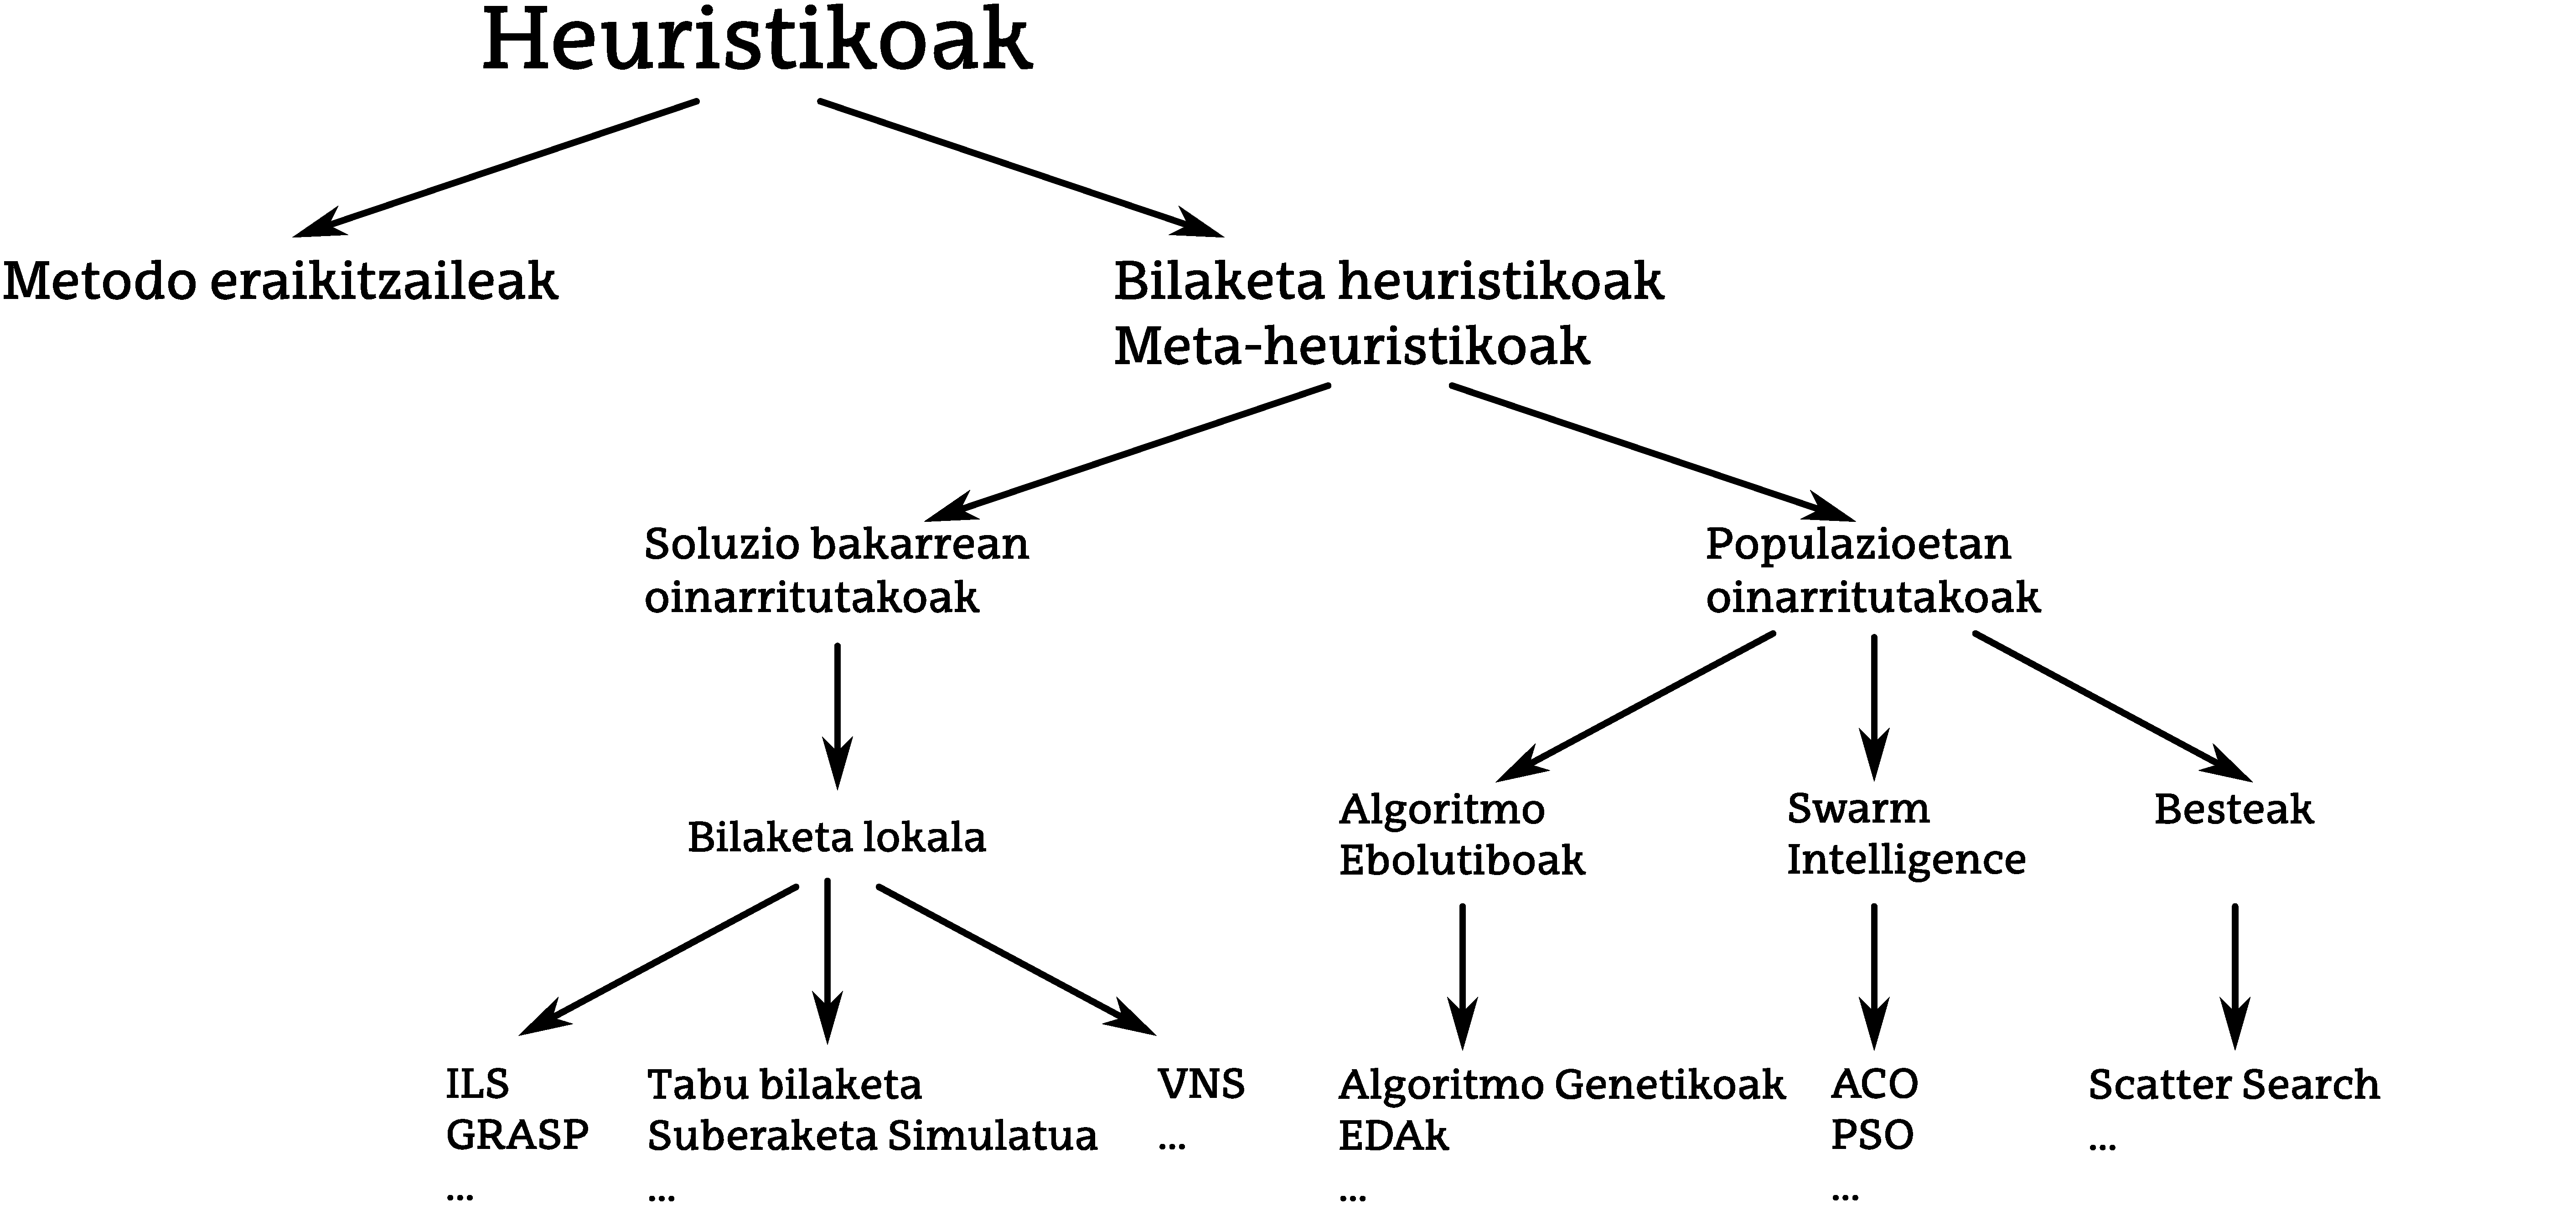
\includegraphics[width=1\linewidth]{./Irudiak/heur_sailkap}
\caption{Metodo heuristikoen eskema}
\label{fig:heur_sailkap}
\end{figure}

\ref{fig:heur_sailkap} irudian optimizaziorako heuristikoen eskematxo bat ikus daiteke. Meta-heuristiko asko daude baina denak gauza berdina egiteko diseinatuta daude: bilaketa espazioa miatzeko. Miaketa prozesuan bi estrategia ezberdin erabil --eta, batez ere, konbina-- daitezke: \textit{dibertsifikazioa} eta \textit{areagotzea}. Dibertsifikatzean espazioko eremu handiak aztertzen ditugu, baina xehetasun handirik gabe; helburua bilaketa espazioko eremu interesgarriei antzematea da --espazioa esploratzea, alegia--. Areagotzeak, berriz, topatu ditugun eremu interesgarri horiek sakonki arakatzea dauka helburutzat; batzuetan esaten den legez, soluzio onak esplotatzea. Oro har, bilaketa lokala motako algoritmoetan areagotzeari garrantzi handiagoa ematen zaio; populazioetan oinarritutako algoritmoetan, berriz, dibertsifikazioa da helburu nagusia\footnote{Izan ere, azken kapituluan ikusiko dugun bezala, teknikak nahas daitezke, bilaketa lokalean oinarritutako areagotze pausuak populazioetan oinarritutako metodoei gehituz}.

Txantiloiak edo eskemak definitzeko behar den abstrakzio maila lortzeko \textit{operadoreak} --soluzioak maneiatzeko erabiltzen diren funtzio matematikoak-- erabiltzen dira. Adibide gisa, bilaketa lokalean, \textit{ingurune operadoreak} erabiltzen dira; hau da, soluzio bat emanda, soluzio horren \zkk antzerakoak\skk\ diren soluzioak itzultzen dituen operadore edo funtzioa. Datorren kapituluan ikusiko dugun bezala, algoritmoa definitzeko ez zaigu axola, problema konkretu batean, zein ingurune funtzioa erabiltzen den, bakarrik jakin behar dugu soluzio bat dugunean bere ingurunean dauden soluzioak emango dizkigun operadorea izango dugula.

%\subsection{Parametroen egokitzapena}

%Hurrengo kapituluetan aurkeztuko diren algoritmoek hainbat parametro izango dituzte; are gehiago, parametro hauek algoritmoen performantzian eragin handia izan dezakete. Hori dela eta, problema bat ebazterakoan, behin metaheuristikoa diseinaturik dugula, bere parametroak egokitu egin behar dira, albait soluziorik onena topatzeko.

%Parametroak egokitzeko esperimentu konputazionalak diseinatu behar ditugu, algoritmoen portaera parametro konbinazio ezberdinekin ebaluatzeko. Esperimentuak diseinatzeko lehendabiziko gauza egokitu behar diren parametroei antzematea da. Behin parametro guztiak zerrendatuta, bakoitzak zein balioa har ditzakeen jakin behar dugu; parametro batzuk jarraituak izango dira --probabilitateak, adibidez--, eta beste batzuk kategorikoak. Hau kontuan harturik, parametro bakoitzeko zein balioak testatuko ditugun erabaki beharko dugu.

%Parametro bakoitzeko erabiliko ditugun balioen kopuruak oso garrantzitsuak dira, esperimentazioaren tamainan eragin handia izango baitute. Demagun gure algoritmoak hiru parametro numeriko dituela eta bakoitzeko bi balio testatu nahi ditugula; guztira zortzi esperimentu egin beharko ditugu, bat hiru parametroen konbinaketa bakoitzeko. Alabaina, parametroen bi balio barik lau testatu nahi baditugu, 64 esperimentu exekutatu beharko genituzke. Izan ere, diseinu esperimental honi \textit{full factorial} deritzo, eta esperimentu kopurua esponentzialki hazten da parametro kopuruarekiko. Parametro gutxi ditugunean hurbilketa hau egokia izan arren, hainbat kasutan bideraezina gertatuko da. Konbinazio guztiak probatzerik ez badago, beste hainbat aukera ditugu. Sinpleena, parametroak independienteki egokitzea da; beste hurbilketa aurreratuagoetan konbinaketa guztietatik batzuk aukeratzeko irizpideak erabiltzen dira --\zkk latin hypercube\skk \cite{mckay1979} deritzona, esate baterako--.

%\begin{figure}[t]
%\centering
%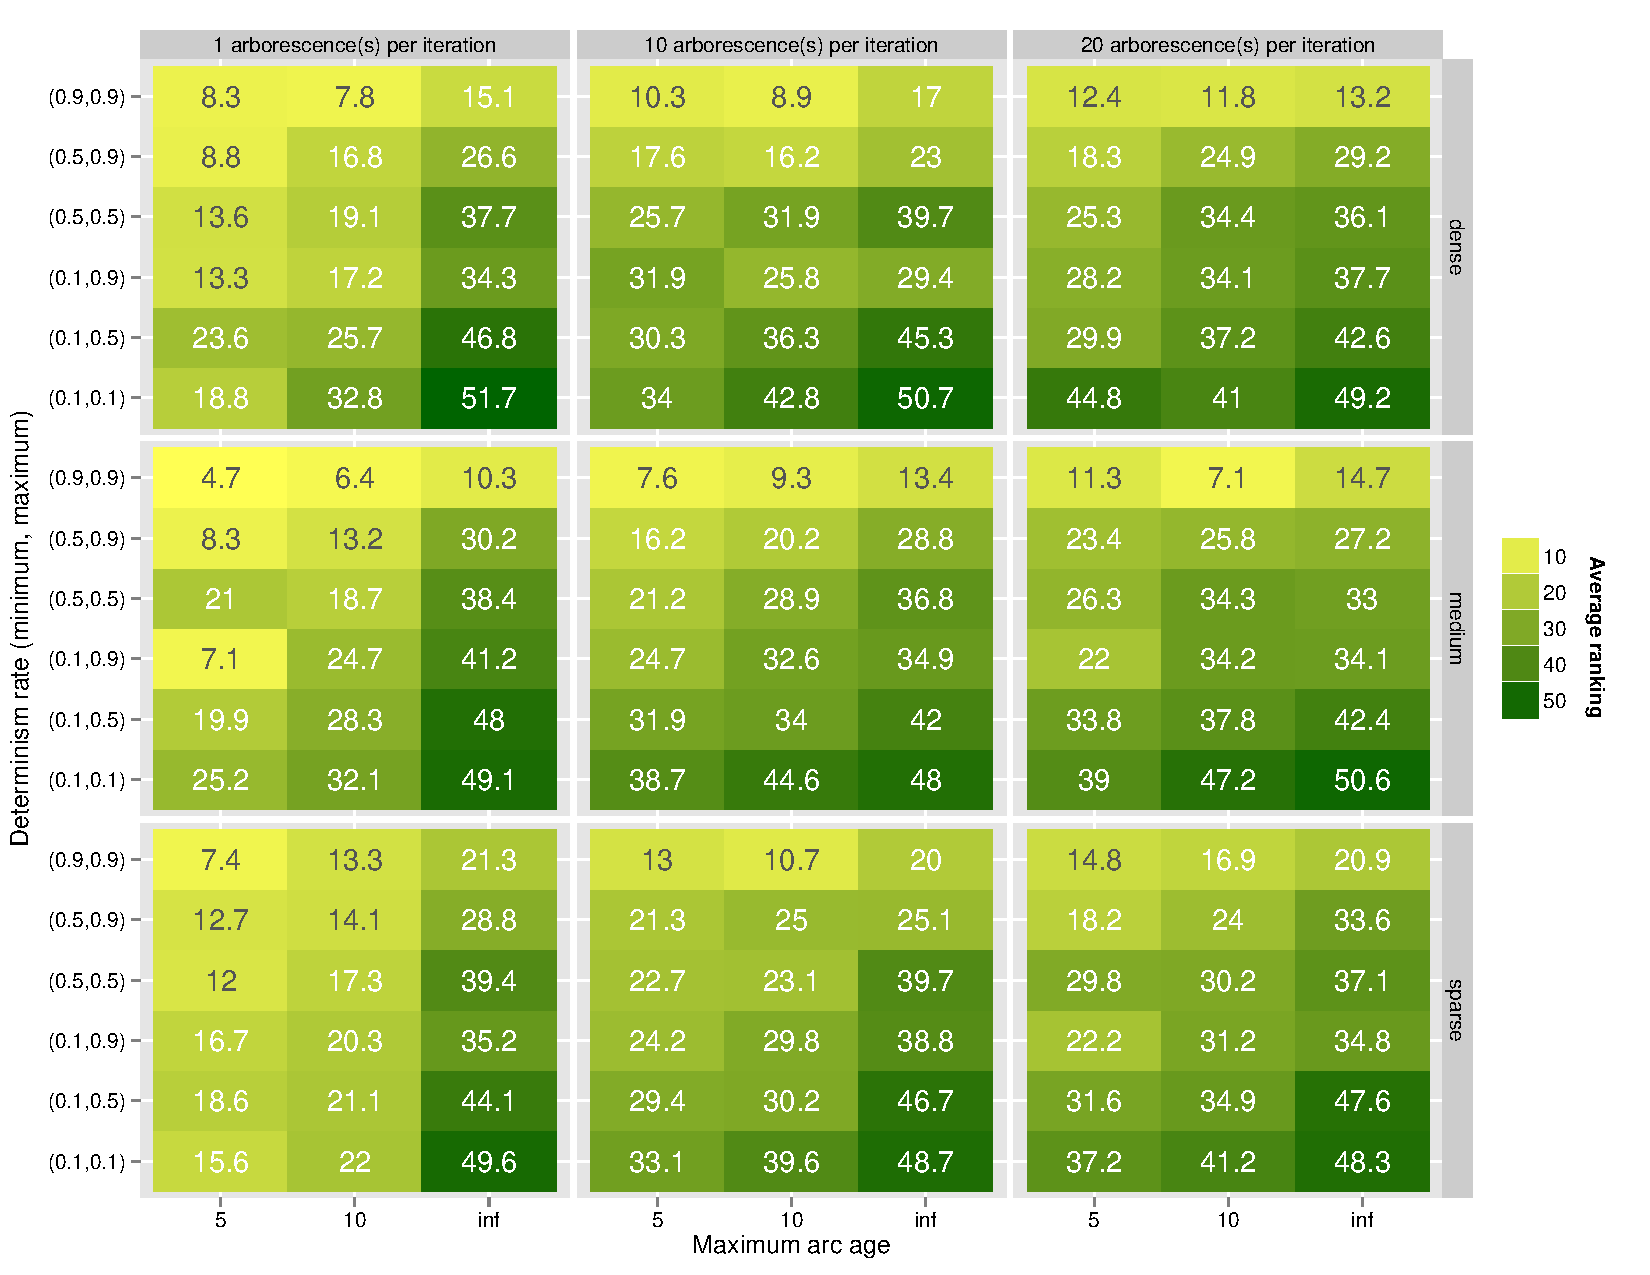
\includegraphics[width=\linewidth]{./Irudiak/data_tuning_dg}
%\caption{Parametroen egokitzapenerako egindako esperimentuen bistaratzearen adibide bat. Adierazpide hau erabiliz lau parametroen eragina azter daiteke grafiko bakar batean}
%\label{fig:parametroen_egokitzapena}
%\end{figure}

%Behin esperimentazioa diseinaturik, exekutatu, emaitzak jaso eta interpretatu egin behar dira. Emaitzak aztertzerakoan taulak erabilera oso hedatua egon arren, grafikoak egokiagoak izan ohi dira, parametro konbinazio onenei errazago antzematen baitzaie. \ref{fig:parametroen_egokitzapena} irudian kasu erreal batean egindako esperimentazioaren emaitzak ikus daitezke. Adierazpide hau erabiliz lau parametroen eragina grafiko bakar batean ikus daiteke. Azpi-grafiko bakoitzean $X$ ardatzean 3 balio hartzen dituen parametro bat, \textit{maximum arc age} deritzona, adierazten da. $Y$ ardatzean berriz, \textit{determinism rate} parametroa adierazten da, zeinek sei balio hartzen ditu\footnote{Izanez, ardatz honek bi parametro adierazten ditu, balio maximoa eta minimoa. Bakoitzari hiru balio posible esleituz (0.1, 0.5 eta 0.9), parametroen interpretazioa dela eta bakarrik sei konbinazio dira zentzua dutenak, balio minimoa ezin baita izan maximoa baino handiagoa}. Bi parametro hauetaz gain beste bi aztertzen dira. Azpi-grafikoak ordenatuta daude, errenkada berdinean dentsitate berdina (\textit{dense}, \textit{medium} eta \textit{sparse}) dutenak jarriz eta zutabe bakoitzean \textit{arborescences per iteration} balio berdina dutenak. Guztira, grafikoan 162 ($3\cdot 6\cdot 3\cdot 3)$ esperimentuen emaitzak bistaratzen dira. Balioa emateaz gain koloreak erabiltzen dira konbinazio onenak nabarmentzeko eta emaitzetan dauden patroiei errazago antzemateko\footnote{Izan ere, koloreak kentzen baditugu emaitza taula bat besterik ez da!}.

%Parametroak egokitzeko estrategia honi \textit{off-line} deritzo, optimizazio algoritmoa exekutatu aurretik egiten baita. \textit{On-line} optimizazioan, berriz, parametroak algoritmoaren exekuzioan zehar egokitzen dira, areagotzea eta dibertsifikazioa kontrolatzeko, adibidez. 

%Problema konkretu bat ebazteko parametro konbinaziorik onena bilatu nahi badugu, egokitzapena bera optimizazio problema bat moduan ikus dezakegu eta, hortaz, optimizazio algoritmo bat erabil dezakegu parametroak optimizatzeko. Ideia honi meta-optimizazioa deritzo eta parametroak optimizatzeko erabiltzen diren algoritmoei, berriz, meta-metaheuristikoak.


\bibliographystyle{plain}
\bibliography{references}


\end{document}

